\chapter{Interpolation of Unitaries with Time-Dependent Hamiltonians via Deep Learning}
\label{ch:results-pinn-unitaries}

This chapter presents the first main application developed in this thesis: a physics-informed deep learning framework for estimating the unitary time-evolution operator of quantum systems governed by time-dependent Hamiltonians over a full time domain. The results reported here correspond to the work submitted for publication in \textit{Machine Learning: Science and Technology}~\cite{guerra2026interpolation}.

The theoretical background required for this chapter was developed in Chapter~\ref{sec:quantum_information}: the von Neumann equation~\eqref{eq:von_neumann} and its formal solution in terms of the time-ordered exponential~\eqref{eq:time_ordered_exponential}, the Magnus expansion~\eqref{eq:magnus}, the Trotter product formula~\eqref{eq:trotter}, the Pauli-basis representation of $N$-qubit operators (Section~\ref{sec:pauli_basis}), and the gate fidelity~\eqref{eq:gate_fidelity} between unitary channels obtained through the Choi--Jamio\l{}kowski isomorphism~\eqref{eq:choi}. The deep learning machinery --- fully connected architectures~\eqref{eq:fully-connected-network}, loss functions (Section~\ref{sec:loss_functions}), gradient-based optimization (Section~\ref{sec:optimization}), and the physics-informed paradigm (Section~\ref{sec:pinns}) --- was introduced in Chapter~\ref{sec:deep_learning}. In accordance with Chapter~\ref{sec:quantum_information}, natural units with $\hbar = 1$ are used throughout this chapter.

%-----------------------------------------------------------
\section{Problem statement}
\label{sec:res-problem}

A fundamental challenge in quantum theory is the accurate modeling of the dynamics of quantum systems driven by time-dependent Hamiltonians. Unlike the time-independent case, where the time-evolution operator reduces to a simple matrix exponential $e^{-iHt}$, time-dependent Hamiltonians give rise to the time-ordering operator, which precludes a closed-form solution and introduces substantial mathematical and numerical complexity. The cost of any direct approach is further compounded by the exponential growth of the Hilbert space~\cite{lloyd1996}, together with the rapidly growing number of terms required in the series expansions used to represent the time-dependent evolution operator $U(t)$: for an $N$-qubit system the evolution operator is a $2^N \times 2^N$ matrix, and its dense construction or exponentiation scales as $\mathcal{O}(2^{3N})$. Expansions such as the Dyson or Magnus series, discussed in Chapter~\ref{sec:quantum_information}, involve nested time integrals whose number grows with the expansion order, and the associated numerical errors tend to accumulate over long evolution times~\cite{wiebe_simulating_2011, blanes2009}. Even on quantum hardware, simulating time-dependent dynamics is generally more demanding than the time-independent case, particularly for rapidly varying or highly oscillatory Hamiltonians~\cite{an2022}. Despite these difficulties, time-dependent Hamiltonians play a central role in quantum technologies, including quantum control and gate optimization~\cite{Ansel_2024}, as well as quantum simulation of complex many-body systems~\cite{georgescu2014, cao2025}.

Several approaches have been developed to address this challenge. Methods based on truncated Dyson series expansions have shown promising results in handling the time-ordering operator~\cite{berry_2015, krieferova_2019}. Magnus-expansion-based algorithms have proven particularly effective in quantum control~\cite{Dalgaard_2022}, and recent work has extended these to highly-oscillatory Hamiltonians relevant to near-term quantum devices~\cite{chen_quantum_2023, fang_time-dependent_2024}. Modified Suzuki--Trotter decompositions have been proposed for interpolating unitary operators in time-dependent settings~\cite{schilling2024}. Tensor-network methods provide a complementary route: they enable efficient classical simulation of one-dimensional systems through time-evolving block decimation~\cite{vidal_efficient_2004}, and recent constructions optimize Suzuki--Trotter decompositions for Hamiltonian simulation and adiabatic quantum computing~\cite{tepaske2023, causer2024}. On the machine learning side, PINNs have been explored to learn quantum dynamics under physical constraints~\cite{norambuena2024}, as well as to reconstruct time-dependent Hamiltonians using deep learning models~\cite{che_2021, han_2021}. Other measurement-based protocols have also been proposed for this task~\cite{franceschetto2025}.

The specific problem addressed in this chapter is the following. Starting from the knowledge of the time-evolution operator $U(t_i)$ on a finite set $\{t_i\}$ ($i=1,\dots,N$) of times with $t_i\in[0,T]$, we seek to interpolate $U(t)$ over the entire time interval $[0,T]$. The model takes a single scalar, the time $t$, as input and returns the corresponding time-evolution operator. Crucially, the time-dependent Hamiltonian itself is not provided to the model; it learns the dynamics solely from the sampled unitaries $U(t_i)$ and the associated evolved states. Throughout this chapter, the training data are generated numerically, but are intended to play the role of experimental data that, in practice, would be obtained, for example, by quantum process tomography (QPT). Each model is trained to represent the dynamics of a single Hamiltonian realization; learning a mapping that generalizes across different Hamiltonians is beyond the scope of this work.

In the language of Chapter~\ref{sec:quantum_information}, the available information consists of a known set of discrete data, either evolved states $\left\{ \rho_0, \rho(t_i) \right\}_{i=1}^{N_1}$ or sampled unitaries $\left\{ U(t_j,t_0) \right\}_{j=1}^{N_2}$, where the states evolve according to \textit{Postulate~2}, $\rho(t_i) = U(t_i,t_0)\,\rho_0\,U^{\dagger}(t_i,t_0)$, and the sampled unitaries are solutions of the von Neumann dynamics, see Eq.~\eqref{eq:von_neumann}. From this discrete data the model is trained to reconstruct $U(t)$ over the full interval $[0,T]$.

Our method is based on the PINN framework introduced in Section~\ref{sec:pinns}, in which known physical constraints are explicitly incorporated into the training process to guide the learning of physically consistent solutions. Due to the exponential growth of the Hilbert space with the number of qubits, we train separate models per system size and test two distinct model architectures: (i) a model trained to directly predict the unitary operator $U(t)$, and (ii) a model that predicts the coefficients of an effective time-dependent Hamiltonian $H_\mathrm{eff}(t)$, from which $U(t)$ is subsequently computed via the Magnus expansion or Trotterization. The motivation for the second architecture is scalability: by reducing the task from learning the full unitary to learning an effective Hamiltonian, the number of free parameters is drastically reduced, lowering the computational resources required for training.

%-----------------------------------------------------------
\section{Physical systems}
\label{sec:res-systems}

We consider three types of Hamiltonians across different many-body configurations, all expressed in the $N$-qubit Pauli basis introduced in Section~\ref{sec:pauli_basis}. For systems with up to 6 qubits, we employ the general Hamiltonian containing all possible Pauli components; for systems with 7 or 8 qubits, we restrict the Hamiltonian to two reduced nearest-neighbor models: an Ising model and an $XYZ$ Heisenberg model. These are explicitly given by
\begin{align}
H_{\mathrm{general}}(t)
&=
\sum_{\alpha_1,\ldots,\alpha_N}
c_{\alpha_1 \cdots \alpha_N}(t)\,
\sigma_{\alpha_1}\otimes\cdots\otimes\sigma_{\alpha_N},
\label{eq:res-H-general}
\\
H_{\mathrm{Ising}}(t)
&=
\sum_{j=1}^{N-1}
J_j(t)\,
\sigma_j^z \sigma_{j+1}^z
+
\sum_{j=1}^{N}
h_j(t)\,
\sigma_j^z,
\label{eq:res-H-ising}
\\
H_{XYZ}(t) &= \sum_{j=1}^{N-1} \qty[
J_j^x(t)\, \sigma_j^x \sigma_{j+1}^x
+ J_j^y(t)\, \sigma_j^y \sigma_{j+1}^y
+ J_j^z(t)\, \sigma_j^z \sigma_{j+1}^z ].
\label{eq:res-H-xyz}
\end{align}
Here each index $\alpha_j \in \{ I, x, y, z \}$ labels the Pauli operator acting on the $j$-th qubit, the real-valued coefficients $c_{\alpha_1 \cdots \alpha_N}(t)$ carry the full time dependence, and $\sigma_j^{x,y,z}$ denote the Pauli operators acting on the $j$-th qubit. In the Ising model, $J_j(t)$ is the time-dependent coupling strength between neighboring qubits $j$ and $j+1$, while $h_j(t)$ is the time-dependent longitudinal field acting on qubit $j$. In the $XYZ$ Heisenberg model, $J_j^x(t)$, $J_j^y(t)$, and $J_j^z(t)$ are the time-dependent nearest-neighbor exchange couplings along the $x$, $y$, and $z$ directions, respectively. All coupling and field coefficients are real-valued functions of time. For brevity, we collect the indices into a multi-index $\vec{\alpha} \equiv (\alpha_1, \ldots, \alpha_N)$, so that $c_{\vec{\alpha}}(t) \equiv c_{\alpha_1 \cdots \alpha_N}(t)$ and $\sigma_{\vec{\alpha}} \equiv \sigma_{\alpha_1} \otimes \cdots \otimes \sigma_{\alpha_N}$.

The choice of a fully non-zero Pauli Hamiltonian for systems up to 6 qubits is motivated by its generality: since any $N$-qubit Hamiltonian can be expressed as a linear combination of all Pauli tensor products (cf.~Section~\ref{sec:pauli_basis}), a model capable of reproducing the dynamics generated by such a Hamiltonian should, in principle, be capable of handling any sparser Hamiltonian as a special case. This choice serves as a proof of principle: an architecture expressive enough to represent the dynamics of such a general Hamiltonian is, \textit{a fortiori}, expressive enough to represent that of any sparser, physically motivated Hamiltonian, although each case requires training a dedicated model on its own data. For systems of 7 and 8 qubits, computational constraints required the use of more structured Hamiltonians that are directly relevant to physically realizable systems. The nearest-neighbor Ising model with longitudinal couplings and fields describes the effective spin dynamics in trapped-ion quantum simulators~\cite{Kim2011}, superconducting qubit architectures~\cite{Wu2016}, and quantum annealing devices such as D-Wave processors, where a time-dependent Hamiltonian drives the system toward the ground state of a programmable Ising problem~\cite{Kadowaki1998}. The nearest-neighbor $XYZ$ Heisenberg model describes anisotropic exchange interactions present in magnetic materials~\cite{Coldea2001}, has been experimentally realized in trapped-ion chains~\cite{Kim2012, Grass2014}, and serves as the effective low-energy Hamiltonian in silicon spin-qubit platforms~\cite{Zajac2018} and nuclear magnetic resonance quantum processors~\cite{Zhang2005}.

For all cases, the time-dependent coefficients take the form
\begin{equation}
\label{eq:res-coeff-form}
c_{\vec{\alpha}}(t) = \frac{A_{\vec{\alpha}} \sin(\omega_{\vec{\alpha}}\, t + \phi_{\vec{\alpha}})}{\mathcal{N}_N},
\end{equation}
where $A_{\vec{\alpha}}$, $\omega_{\vec{\alpha}}$, and $\phi_{\vec{\alpha}}$ are the amplitude, angular frequency, and phase shift of each component, respectively, and $\mathcal{N}_N$ is a system-size-dependent normalization factor introduced to control the operator norm of the Hamiltonian, ensuring the convergence of the Magnus expansion (see Section~\ref{sec:res-integration}). The parameters are independently drawn from uniform distributions: $\omega_{\vec{\alpha}}, \phi_{\vec{\alpha}} \in [0, 2\pi)$ and $A_{\vec{\alpha}} \in [0, 1)$. Once fixed for a given realization, they remain constant throughout training. The same functional form is used for the coupling and field coefficients of the Ising and $XYZ$ systems.

The number of independent coefficients depends on the Hamiltonian structure: $4^N-1$ for the general Pauli case (the global identity component is fixed to zero, see below), $2N-1$ for the Ising model, and $3(N-1)$ for the $XYZ$ model. The normalization factors are
\begin{equation}
\mathcal{N}_2 = 2,\quad \mathcal{N}_3 = 3,\quad \mathcal{N}_4 = 4,\quad \mathcal{N}_5 = 16,\quad \mathcal{N}_6 = 24,
\end{equation}
for the general Pauli Hamiltonian, $\mathcal{N}_7 = \mathcal{N}_8 = 2$ for the Ising, and $\mathcal{N}_7 = \mathcal{N}_8 = 3$ for the $XYZ$ systems, reflecting the smaller number of non-zero terms in the latter cases. Additionally, the coefficient associated with the global identity operator is set to zero in all cases, ensuring that the Hamiltonian is traceless.

The use of randomly sampled parameters allows the generation of a diverse ensemble of time-dependent Hamiltonians, preventing overfitting to specific dynamical patterns and enabling a systematic assessment of the model's ability to generalize across a broad class of physically valid quantum systems.

%-----------------------------------------------------------
\section{Model description}
\label{sec:res-model}

The rationale for employing PINNs lies in their capability to incorporate physical and mathematical constraints directly into the training process. As discussed in Chapter~\ref{sec:deep_learning}, PINNs have demonstrated outstanding performance in solving nonlinear differential equations and in modeling complex dynamical systems~\cite{Raissi2019, karniadakis2021}. Furthermore, neural networks consistently exhibit advantages in interpolation accuracy and adaptability to complex boundary and initial condition constraints.

We employ a model that generates a unitary complex-valued matrix from a scalar input. The number of complex entries of these matrices increases exponentially with the number of qubits as $4^N$. Figure~\ref{fig:res-scalability} shows the number of trainable parameters for models up to 6 qubits, as well as the estimated parameter counts required for 7- and 8-qubit systems. Since the optimization process becomes computationally intractable at larger scales, an alternative strategy is adopted for these higher-dimensional cases. Rather than merely constraining the Hamiltonian to a reduced set of components, the model is constructed to estimate an effective time-dependent set of coefficients defining the effective Hamiltonian of the system $H_{\mathrm{eff}}(t)$. Subsequently, with a model capable of generating $H_{\mathrm{eff}}(t)$, we can use it to compute the time-evolution operator through (i) the Magnus expansion or (ii) the Trotterization. This approach reduces the number of trainable parameters to approximately $10^3$.

\begin{figure}[htbp]
  \centering
  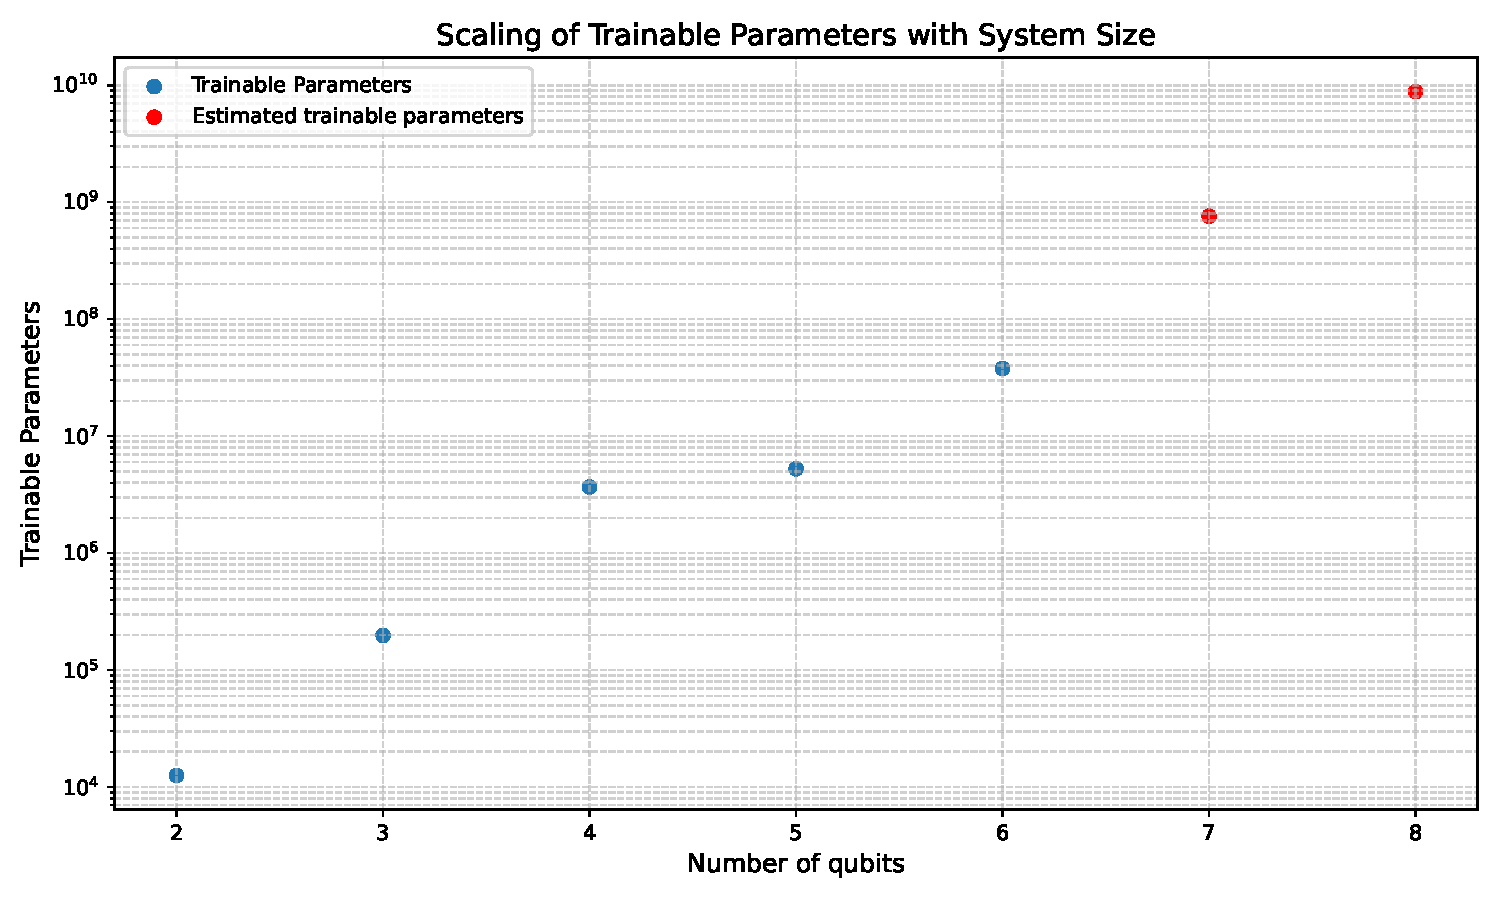
\includegraphics[width=\textwidth]{images/scaling_num-trainable-parameters.pdf}
  \caption[Trainable parameters as a function of the number of qubits]{Amount of trainable parameters as a function of the number $N$ of qubits. In cases with up to 6 qubits, this relationship is outlined. For systems containing 7 and 8 qubits, we have provided the estimated number of trainable parameters required to apply the same strategy to determine the unitary evolution operator for those systems.}
  \label{fig:res-scalability}
\end{figure}

\begin{figure}[htbp]
  \centering
  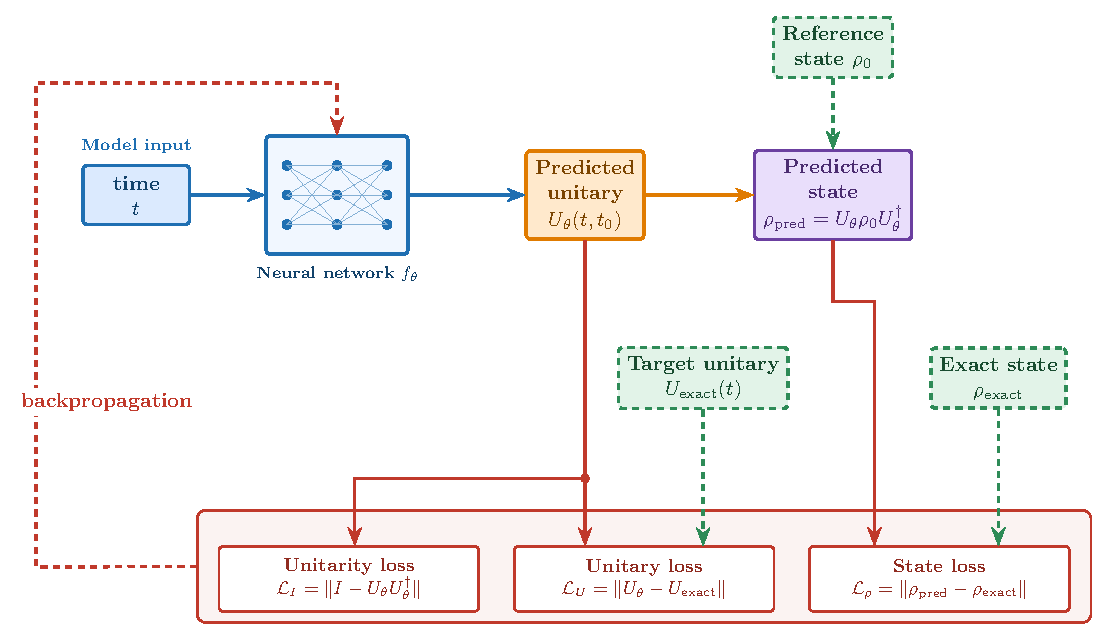
\includegraphics[width=0.99\textwidth]{images/model-description-1.pdf}

  \vspace{1mm}
  {\small (a) PINN model for 2 to 6 qubits.}

  \vspace{5mm}

  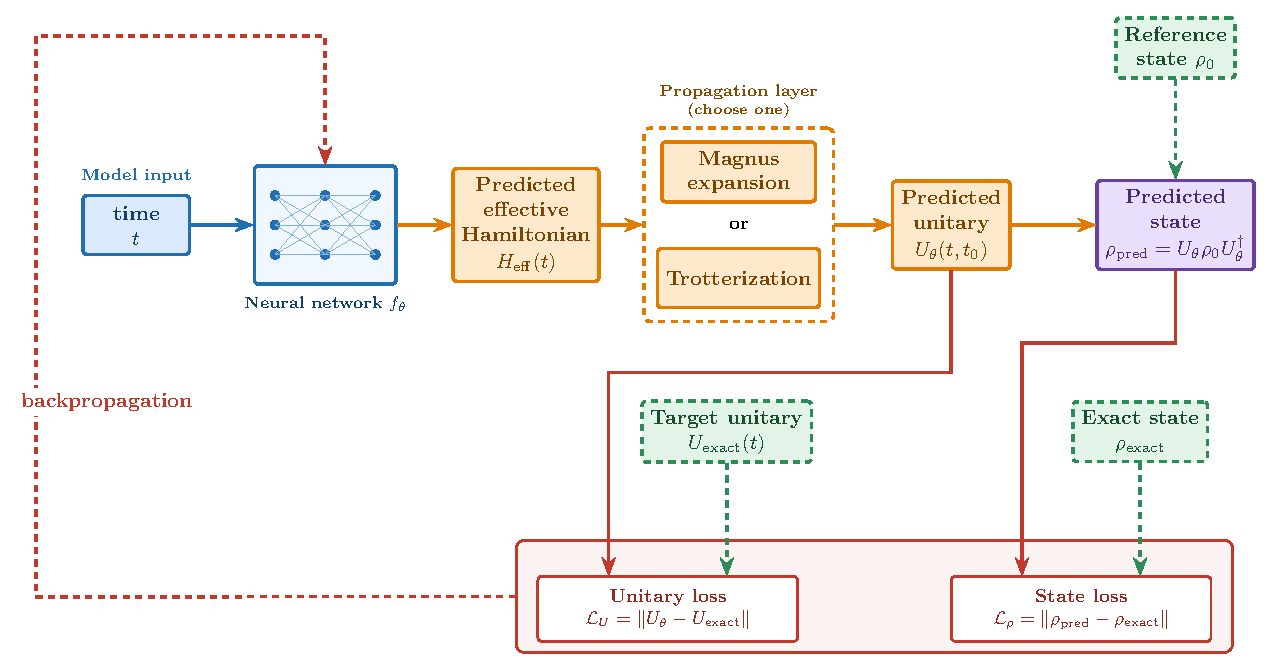
\includegraphics[width=0.99\textwidth]{images/model-description-2.pdf}

  \vspace{1mm}
  {\small (b) PINN model for 7 and 8 qubits.}

  \caption[The two PINN architectures used to emulate the temporal evolution of multi-qubit systems]{The two PINN architectures used to emulate the temporal evolution of isolated multi-qubit systems. The network $f_\theta$ takes time $t$ as input and is trained via backpropagation. (a) For 2--6 qubits, it directly predicts the unitary $U_\theta(t,t_0)$, optimized using unitarity, unitary, and state losses. (b) For 7--8 qubits, it predicts an effective Hamiltonian $H_{\mathrm{eff}}(t)$, which is converted into $U_\theta(t,t_0)$ through a propagation layer; unitarity is therefore guaranteed by construction. Colors: blue, inputs/outputs; orange, learned quantities; purple, predicted state; dashed green, reference and target quantities; red, losses and optimization path.}
  \label{fig:res-models-description}
\end{figure}

\subsection{Architecture description}
\label{sec:res-architecture}

For the model architecture, we employ a straightforward approach consisting of a sequence of fully connected layers (cf.~Section~\ref{sec:neural_networks}) designed to match the number of parameters required for the output matrix. The hyperbolic tangent function is used as the activation function. This architecture can generate arbitrarily complex-valued matrices, ensuring that the model can accurately represent any matrix form of the time-evolution operator. Figure~\ref{fig:res-models-description} schematically illustrates the two modeling strategies adopted for the time-evolution operator.

\paragraph{Cases with 2 to 6 qubits.}
The model's internal data processing involves several fully connected layers. Initially, the input layer takes a scalar input corresponding to time. This input is processed through fully connected layers that progressively increase the dimensionality of the latent representation. After each hidden layer, a hyperbolic tangent activation function is applied. The resulting features are then reshaped into tensors of dimension $(2, 2^N, 2^N)$, where the first index is used to construct the real and imaginary parts of the resulting complex-valued matrix. A detailed description of each architecture is presented in Table~\ref{tab:res-model-architecture}.

\begin{table}[htbp]
\centering
\renewcommand{\arraystretch}{1.2}

% --------- model2 & model3 ----------
\begin{minipage}[t]{0.48\textwidth}
\centering
\textbf{\textit{model2}} (2 qubits)\\[0.5ex]
\begin{tabular}{c|c|c}
\hline
\textbf{Layer} & \textbf{Input} & \textbf{Output} \\
\hline \hline
Linear 1 & 1 & 64 \\
Tanh & - & - \\
Linear 2 & 64 & 128 \\
Tanh & - & - \\
Linear 3 & 128 & 32 \\
Reshape & 32 & $(2,4,4)$ \\
\hline
\end{tabular}
\end{minipage}
\hfill
\begin{minipage}[t]{0.48\textwidth}
\centering
\textbf{\textit{model3}} (3 qubits)\\[0.5ex]
\begin{tabular}{c|c|c}
\hline
\textbf{Layer} & \textbf{Input} & \textbf{Output} \\
\hline \hline
Linear 1 & 1 & 256 \\
Tanh & - & - \\
Linear 2 & 256 & 512 \\
Tanh & - & - \\
Linear 3 & 512 & 128 \\
Reshape & 128 & $(2,8,8)$ \\
\hline
\end{tabular}
\end{minipage}

\medskip

% --------- model4 & model5 ----------
\begin{minipage}[t]{0.48\textwidth}
\centering
\textbf{\textit{model4}} (4 qubits)\\[0.5ex]
\begin{tabular}{c|c|c}
\hline
\textbf{Layer} & \textbf{Input} & \textbf{Output} \\
\hline \hline
Linear 1 & 1 & 512 \\
Tanh & - & - \\
Linear 2 & 512 & 1024 \\
Tanh & - & - \\
Linear 3 & 1024 & 2048 \\
Tanh & - & - \\
Linear 4 & 2048 & 512 \\
Reshape & 512 & $(2,16,16)$ \\
\hline
\end{tabular}
\end{minipage}
\hfill
\begin{minipage}[t]{0.48\textwidth}
\centering
\textbf{\textit{model5}} (5 qubits)\\[0.5ex]
\begin{tabular}{c|c|c}
\hline
\textbf{Layer} & \textbf{Input} & \textbf{Output} \\
\hline \hline
Linear 1 & 1 & 512 \\
Tanh & - & - \\
Linear 2 & 512 & 2048 \\
Tanh & - & - \\
Linear 3 & 2048 & 2048 \\
Reshape & 2048 & $(2,32,32)$ \\
\hline
\end{tabular}
\end{minipage}

\medskip

% --------- model6 ----------
\begin{minipage}[t]{0.48\textwidth}
\centering
\textbf{\textit{model6}} (6 qubits)\\[0.5ex]
\begin{tabular}{c|c|c}
\hline
\textbf{Layer} & \textbf{Input} & \textbf{Output} \\
\hline \hline
Linear 1 & 1 & 1024 \\
Tanh & - & - \\
Linear 2 & 1024 & 4096 \\
Tanh & - & - \\
Linear 3 & 4096 & 8192 \\
Reshape & 8192 & $(2,64,64)$ \\
\hline
\end{tabular}
\end{minipage}

\caption[Architectures of \textit{model2} through \textit{model6}]{Architectures of \textit{model2} through \textit{model6}, each representing the generator of a $2^N \times 2^N$ complex-valued unitary matrix from a scalar temporal input $t$.}
\label{tab:res-model-architecture}
\end{table}

\paragraph{Cases with 7 and 8 qubits.}
For the models handling 7 and 8 qubits, the architecture follows a similar structure to the previous models but differs significantly in the output layer. Instead of generating a complex-valued matrix directly, the output layer produces time-dependent coefficients associated with the Pauli basis representation of the Hamiltonian $H(t)$ (cf.~Section~\ref{sec:pauli_basis}). The output dimension therefore equals the number of independent Hamiltonian coefficients, namely $2N-1$ for the Ising model ($13$ and $15$ for $N=7,8$) and $3(N-1)$ for the $XYZ$ model ($18$ and $21$). A detailed description of these architectures is presented in Table~\ref{tab:res-model-architecture2}, where the output sizes shown correspond to the Ising case.

\begin{table}[htbp]
\centering
\renewcommand{\arraystretch}{1.2}

% --------- model7 & model8 ----------
\begin{minipage}[t]{0.48\textwidth}
\centering
\textbf{\textit{model7}} (7 qubits)\\[0.5ex]
\begin{tabular}{c|c|c}
\hline
\textbf{Layer} & \textbf{Input} & \textbf{Output} \\
\hline \hline
Linear 1 & 1 & 50 \\
Tanh & - & - \\
Linear 2 & 50 & 13 \\
\hline
\end{tabular}
\end{minipage}
\hfill
\begin{minipage}[t]{0.48\textwidth}
\centering
\textbf{\textit{model8}} (8 qubits)\\[0.5ex]
\begin{tabular}{c|c|c}
\hline
\textbf{Layer} & \textbf{Input} & \textbf{Output} \\
\hline \hline
Linear 1 & 1 & 50 \\
Tanh & - & - \\
Linear 2 & 50 & 15 \\
\hline
\end{tabular}
\end{minipage}

\caption[Architectures of \textit{model7} and \textit{model8}]{Architectures of \textit{model7} and \textit{model8}, designed to generate the real-valued coefficients of the Pauli-basis representation of the Hamiltonian from a scalar temporal input $t$. The output sizes shown ($13$ and $15$) correspond to the Ising model ($2N-1$); for the $XYZ$ model the output size is $3(N-1)$, i.e.\ $18$ and $21$ for $N=7,8$.}
\label{tab:res-model-architecture2}
\end{table}

\FloatBarrier

\subsection{Loss function and data generation}
\label{sec:res-loss-function}

To train the model, a valid dataset is required. The dataset generation process is inspired by the idea that it can be interpreted as the outcome of multiple QPT experiments performed at different times~\cite{huang2025}. If the goal is to perform a quantum control task, the dataset will consist of a set of quantum states forming a trajectory and target unitary operators applied at specific times $t$. However, for practical purposes, the dataset is generated numerically by computing the system dynamics: the states evolve according to Eq.~\eqref{eq:postulate2}, and the corresponding unitaries $U(t)$ are obtained from the Trotter product formula~[Eq.~\eqref{eq:trotter}].

Employing the Magnus expansion or the Trotterization method increases the computational cost, as these calculations must be performed at each training iteration to update the model parameters. To mitigate this, the Magnus expansion is truncated at second order. For both the Magnus and Trotterization approaches, we use 50 integration steps per model query, i.e., each time the model produces an output.

Furthermore, a single QPT is insufficient to accurately characterize $U(t)$. In principle, achieving near-perfect fidelities over a continuous time domain would require an infinite number of QPTs due to its continuous nature. Nevertheless, models such as the one proposed here help to reduce the required measurement cost. The study focuses on the time interval $t \in [0, 1]$, employing discrete time grids with step sizes of $\Delta t = 0.1, 0.25, 0.5$, and $1.0$. This procedure yields a comprehensive dataset for the selected time values, essential for effective model training. A training dataset $\left\{ \left( \rho_0^i, \tau_i, \rho_{\tau_i}^i, U_{\tau_i} \right) \right\}_{i=1}^{N_{\mathrm{train}}}$, with $N_{\mathrm{train}} = 11000$, was generated, where the target unitaries $U_{\tau_i}$ are known and the evolved states satisfy $\rho_{\tau_i}^i = U(\tau_i,0)\, \rho_0^i\, U^{\dagger}(\tau_i,0)$. The evolution times $\tau_i \in [0,1]$ are sampled from uniform time grids corresponding to different choices of the time step $\Delta t$. The initial states $\rho_0^i$ are random mixed states sampled from the Hilbert--Schmidt measure~\cite{zyczkowski2001}: a complex matrix $G$ with independent Gaussian real and imaginary entries is drawn, and the state is obtained as $\rho_0 = G G^\dagger / \Tr(G G^\dagger)$, which is Hermitian, positive semi-definite, and normalized by construction.

The loss function is defined as an objective function whose minimization yields the optimal parameters of the deep learning model, such that the resulting model accurately describes the dynamics of the physical system under consideration. It is constructed to explicitly incorporate the known physical constraints governing the system dynamics, as well as the available supervision data. In particular, it enforces consistency with the unitary evolution of states (\textit{Postulate~2}, Eq.~\eqref{eq:postulate2}), agreement with known unitary operators when available, and the unitarity of the predicted time-evolution operator. The total loss function is defined as
\begin{align}
  \label{eq:res-loss}
  \mathcal{L} ={}& \frac{1}{N_{\mathrm{train}}} \sum_{i=1}^{N_{\mathrm{train}}} \qty( \norm{ \rho_{\tau_i}^i - U_{\theta}(\tau_i)\, \rho_0^i\, U_{\theta}^{\dagger}(\tau_i) }
  + \norm{ U_{\theta}(\tau_i) - U_{\tau_i} } ) \nonumber \\
  & + \frac{1}{N_f} \sum_{k=1}^{N_f} \norm{ \id - U_{\theta}(t_k)\, U_{\theta}^{\dagger}(t_k) },
\end{align}
where $\norm{A} = \sum_{ij} |a_{ij}|$ denotes the element-wise $\ell_1$ matrix norm for any matrix $A = [a_{ij}]$, and $U_{\theta}(t)$ represents a neural network parametrization of the time-evolution operator with trainable weights $\theta = \{ \theta_i \}$. As discussed in Section~\ref{sec:pinns}, Physics-Informed Neural Networks employ such neural representations to approximate unknown physical quantities while enforcing governing equations and constraints directly through the loss function~\cite{Raissi2019}.

Here, $N_{\mathrm{train}}$ denotes the number of available state--unitary training pairs, while $N_f$ corresponds to the number of temporal collocation points used to enforce unitarity across the time domain. The first term of the loss enforces accurate quantum state evolution under the predicted unitary operator $U_{\theta}$. The second term promotes consistency between the predicted unitaries and known target unitaries, when such information is available. The third term explicitly imposes the physical constraint of unitarity by penalizing deviations from $U_{\theta}(t) U_{\theta}^{\dagger}(t) = \id$ at arbitrary times.

For the 7- and 8-qubit systems, only the first two terms are employed. This choice is motivated by the fact that both the Magnus expansion and the Trotterization intrinsically preserve unitarity, rendering an explicit unitarity penalty unnecessary in these cases. During training, both methods use $r = 50$ integration steps. Although all results presented in this chapter are obtained using the full loss function in Eq.~\eqref{eq:res-loss}, we observe that satisfactory model performance can be achieved using only a subset of these terms (a quantitative assessment of the role of the unitarity term is presented in Section~\ref{sec:res-unitarity-term}). In this study, we focus on the most favorable training scenario, in which both the target unitary operators and the corresponding evolved quantum states are available during training.

\subsection{Numerical integration of the effective Hamiltonian}
\label{sec:res-integration}

For systems of 7 and 8 qubits, the network $f_\theta$ outputs the Pauli-basis coefficients of an effective Hamiltonian $H_\mathrm{eff}(t)$, and a propagation layer maps it to the time-evolution operator. Two numerical methods are used for this purpose, both of which guarantee exact unitarity of the output by construction; their theoretical foundations were presented in Section~\ref{sec:quantum-dynamics}, and here we describe their discrete numerical implementation.

\paragraph{Second-order Magnus expansion.}
Given a target time $t$ and a number of integration steps $r$, a uniform time grid $\{t_k\}_{k=0}^{r-1}$ is constructed over $[0, t]$ with step size $\Delta t = t/r$. The neural network $f_\theta$ is evaluated at each grid point to obtain the sequence of Hamiltonians $\{H(t_k)\}_{k=0}^{r-1}$. The Magnus operator is truncated up to second order, $\Omega(t) \approx \Omega_1(t) + \Omega_2(t)$, then the time-evolution operator is recovered as
\begin{equation}
    U(t) \approx \exp\qty(-i\, \left[ \Omega_1(t) + \Omega_2(t) \right]).
\end{equation}

The full procedure is summarized in Algorithm~\ref{alg:res-magnus}.

\begin{algorithm}[htbp]
\caption{Second-order Magnus expansion}
\label{alg:res-magnus}
\begin{algorithmic}[1]
\REQUIRE Model $f_\theta$, target time $t$, operator basis $\{\sigma_\mu\}$,
         number of steps $r$
\ENSURE Unitary operator $U(t) \in \mathrm{SU}(d)$
\STATE $\Delta t \leftarrow t / r$
\FOR{$k = 0$ \TO $r-1$}
    \STATE $t_k \leftarrow k\,\Delta t$
    \STATE $\bm{c}_k \leftarrow f_\theta(t_k)$ \COMMENT{model forward pass}
    \STATE $H(t_k) \leftarrow \sum_\mu c_k^\mu\,\sigma_\mu$ \COMMENT{reconstruct Hamiltonian}
\ENDFOR
\STATE $\Omega_1 \leftarrow \sum_{k=0}^{r-1} H(t_k)\,\Delta t$
\STATE $\Omega_2 \leftarrow \mathbf{0}$
\FOR{$m = 0$ \TO $r-1$}
    \FOR{$n = 0$ \TO $m-1$}
        \STATE $\Omega_2 \leftarrow \Omega_2
            - \frac{i}{2}\comm{H(t_m)}{H(t_n)}\Delta t^2$
    \ENDFOR
\ENDFOR
\STATE $U(t) \leftarrow \exp\qty(-i\,(\Omega_1 + \Omega_2))$
\RETURN $U(t)$
\end{algorithmic}
\end{algorithm}

\paragraph{Trotterization.}
Another path to compute the unitary from a given Hamiltonian is by using the Trotterization, described along the Eq.~\eqref{eq:trotter}. Here, by discretizing the time interval into $r$ subintervals of equal length $\Delta t = t/r$ and freezing the Hamiltonian within each slice, we are able to approximate a unitary matrix that, as $r \to \infty$, converges to the exact unitary that we are looking for. To improve accuracy over simple left-endpoint sampling, the Hamiltonian is evaluated at the midpoint of each subinterval,
\begin{equation}
    t_k = \qty(k + \frac{1}{2})\frac{t}{r},
    \quad k = 0, 1, \ldots, r-1.
\end{equation}
Since each factor $\exp(-i H(t_k)\Delta t)$ is exactly unitary, their product is also exactly unitary regardless of the step size, which is the key practical advantage of this method. The full procedure is summarized in Algorithm~\ref{alg:res-trotter}.

\begin{algorithm}[htbp]
\caption{Trotterization}
\label{alg:res-trotter}
\begin{algorithmic}[1]
\REQUIRE Model $f_\theta$, target time $t$, operator basis $\{\sigma_\mu\}$,
         number of steps $r$
\ENSURE Unitary operator $U(t) \in \mathrm{SU}(d)$
\STATE $\Delta t \leftarrow t / r$
\STATE $U \leftarrow \mathbf{I}_d$
\FOR{$k = 0$ \TO $r-1$}
    \STATE $t_k \leftarrow \qty(k + \frac{1}{2})\Delta t$
           \COMMENT{midpoint sampling}
    \STATE $\bm{c}_k \leftarrow f_\theta(t_k)$
           \COMMENT{model forward pass}
    \STATE $H(t_k) \leftarrow \sum_\mu c_k^\mu\,\sigma_\mu$
    \STATE $U_k \leftarrow \exp\qty(-i\,H(t_k)\,\Delta t)$
    \STATE $U \leftarrow U_k\,U$
           \COMMENT{left-multiply to preserve time ordering}
\ENDFOR
\RETURN $U$
\end{algorithmic}
\end{algorithm}

In both methods, $r = 50$ integration steps are used during training and $r = 10$ steps at inference time, since the neural network outputs a smooth effective Hamiltonian for which high temporal resolution is not required at evaluation time.

\subsection{Test and training}
\label{sec:res-test-train}

The AdamW optimizer is used for training, initialized with a learning rate of $10^{-3}$. To enhance convergence stability, a learning-rate scheduler decreases the rate by a factor of $10^{-1}$ every 300 epochs. The training process spans $10^3$ epochs, each consisting of 100 data batches with a batch size of 10. Each dataset contains $11000$ uniformly distributed tuples in the specified time intervals. In addition, the data batches used to train the models for 7- and 8-qubit systems are reduced to 10 data batches per epoch. All models presented in this chapter were trained using an NVIDIA Quadro P6000 GPU. For all model sizes, we observe that datasets with a larger $\Delta t$ yield a more pronounced decrease in the training loss, since the data are less constrained and contain fewer distinct evolution times. We emphasize, however, that a lower training loss does not by itself imply better interpolation: our goal is to predict the unitary at times not seen during training, and a more constrained dataset (smaller $\Delta t$) consistently yields better interpolation accuracy, as quantified by the test-set metrics reported in Section~\ref{sec:res-results}. The full training-loss curves for all system sizes and training configurations are available in the public repository accompanying this work.\footnote{\url{https://github.com/guerra-antonio/PINN_dynamics_estimation}}

%-----------------------------------------------------------
\section{Results}
\label{sec:res-results}

To assess the model's performance over the entire time domain we compute 100 target unitary matrices. These matrices are uniformly spaced in time and include values not present in the training set, thereby allowing us to rigorously evaluate the model's interpolation capability. To quantify accuracy, we adopt the gate fidelity~\cite{cabrera2011} derived in Section~\ref{sec:fidelity} from the Choi--Jamio\l{}kowski representation,
\begin{equation}
  \label{eq:res-metric-fidelity}
  F(U(t), U_{\theta_{\mathrm{opt}}}(t)) = \abs{ \frac{1}{d} \Tr\qty[ U^{\dagger}(t)\, U_{\theta_{\mathrm{opt}}}(t) ] }^2,
\end{equation}
where $\theta_{\mathrm{opt}}$ are the optimal weights of the neural network found during training, and $d = 2^N$ denotes the Hilbert-space dimension for an $N$-qubit system. The fidelity ranges from 0 to 1, with $F = 1$ only when the predicted operator $U_{\theta_{\mathrm{opt}}}(t)$ coincides with the target $U(t)$ at time $t$, up to a global phase.

For evaluation, each trained model generates unitary matrices at the same 100 time points. These predicted matrices are then compared one-by-one with the target unitaries, yielding a fidelity function $F(t)$. Since multiple models for each system size are trained with different values of $\Delta t$, four fidelity curves $F(t)$ are obtained for each system size.

\subsection{Gate fidelity across system sizes}
\label{sec:res-fidelity}

The loss function additionally enforces unitarity across the time domain, ensuring that the model's predictions remain close to unitary transformations throughout training. To further minimize numerical deviations, we can compute the closest unitary matrix to each predicted output via Singular Value Decomposition (SVD), redefining the estimated unitary as
\begin{equation}
  \label{eq:res-error-correction}
  U_{\theta_{\mathrm{opt}}}(t) = U V_{\mathrm{h}},
\end{equation}
where $U$ and $V_{\mathrm{h}}$ arise from the SVD of the model's predicted matrix. The following results compare the performance of the different models with and without post-processing, showing that high fidelity is preserved even in the absence of the closest-unitary correction.

The results in Fig.~\ref{fig:res-fid-2to6} summarize the fidelity performance for systems up to 6 qubits with and without the error correction via Eq.~\eqref{eq:res-error-correction}. As expected, datasets with smaller time steps ($\Delta t$) achieve the highest fidelities due to their finer temporal resolution. Nevertheless, even for larger $\Delta t$, the reduction in fidelity remains minimal. This reflects the PINN's strong interpolation capability, which maintains an accurate approximation of the quantum dynamics even with coarse temporal discretization.

For the 7- and 8-qubit cases, the model follows a different strategy by estimating an effective Hamiltonian as an intermediate step to compute the corresponding unitary matrix. Since evolution can be achieved through Trotterization or Magnus expansion, both approaches were implemented and evaluated independently without SVD post-processing, as both methods guarantee unitarity. Figures~\ref{fig:res-fid78} and~\ref{fig:res-fid78xyz} show the fidelity results for these higher-dimensional systems across different training datasets, for the Ising and $XYZ$ Hamiltonians respectively. Consistent with the behavior observed in Fig.~\ref{fig:res-fid-2to6}, even for large values of $\Delta t$, the degradation in fidelity is minimal, demonstrating that the interpolation remains highly effective in all tested scenarios.

\begin{figure}[htbp]
  \centering
  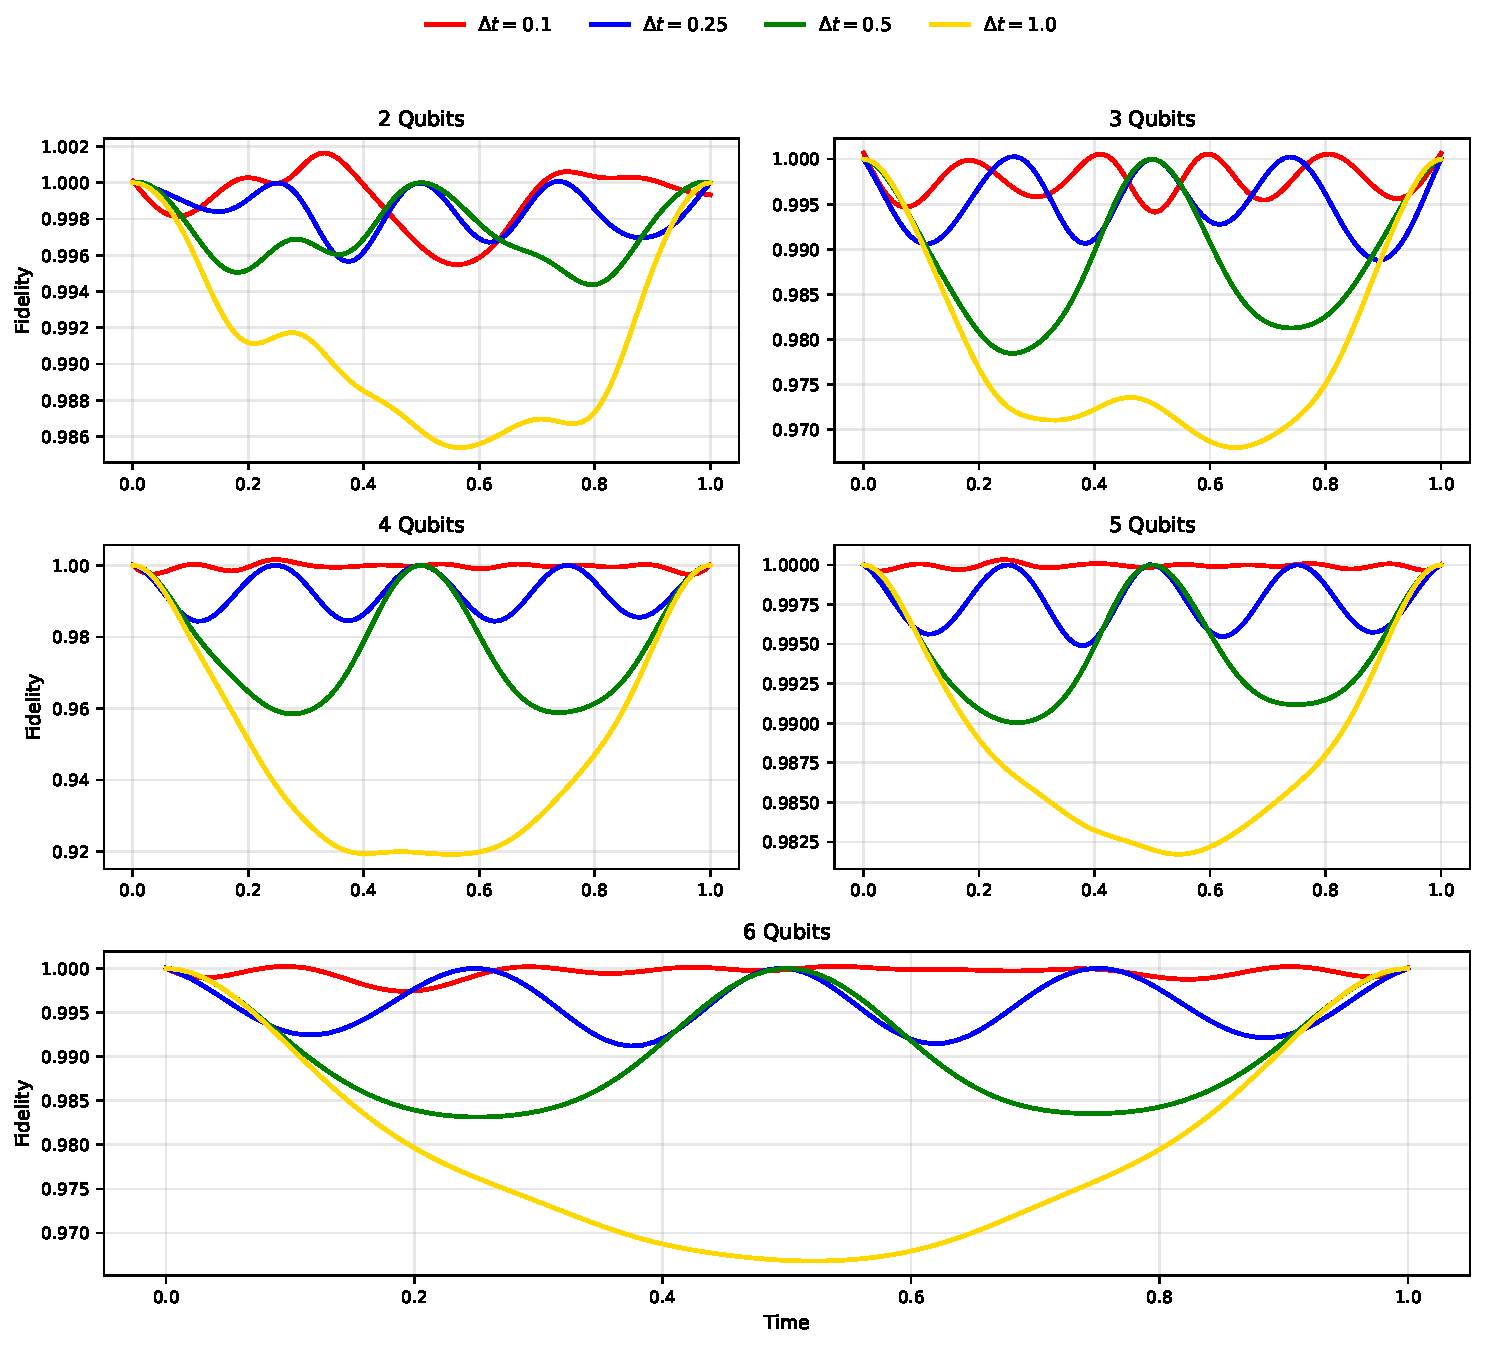
\includegraphics[width=0.8\textwidth]{images/fidelity_qubits_2to6-without.pdf}
  {\small (a)}

  \medskip

  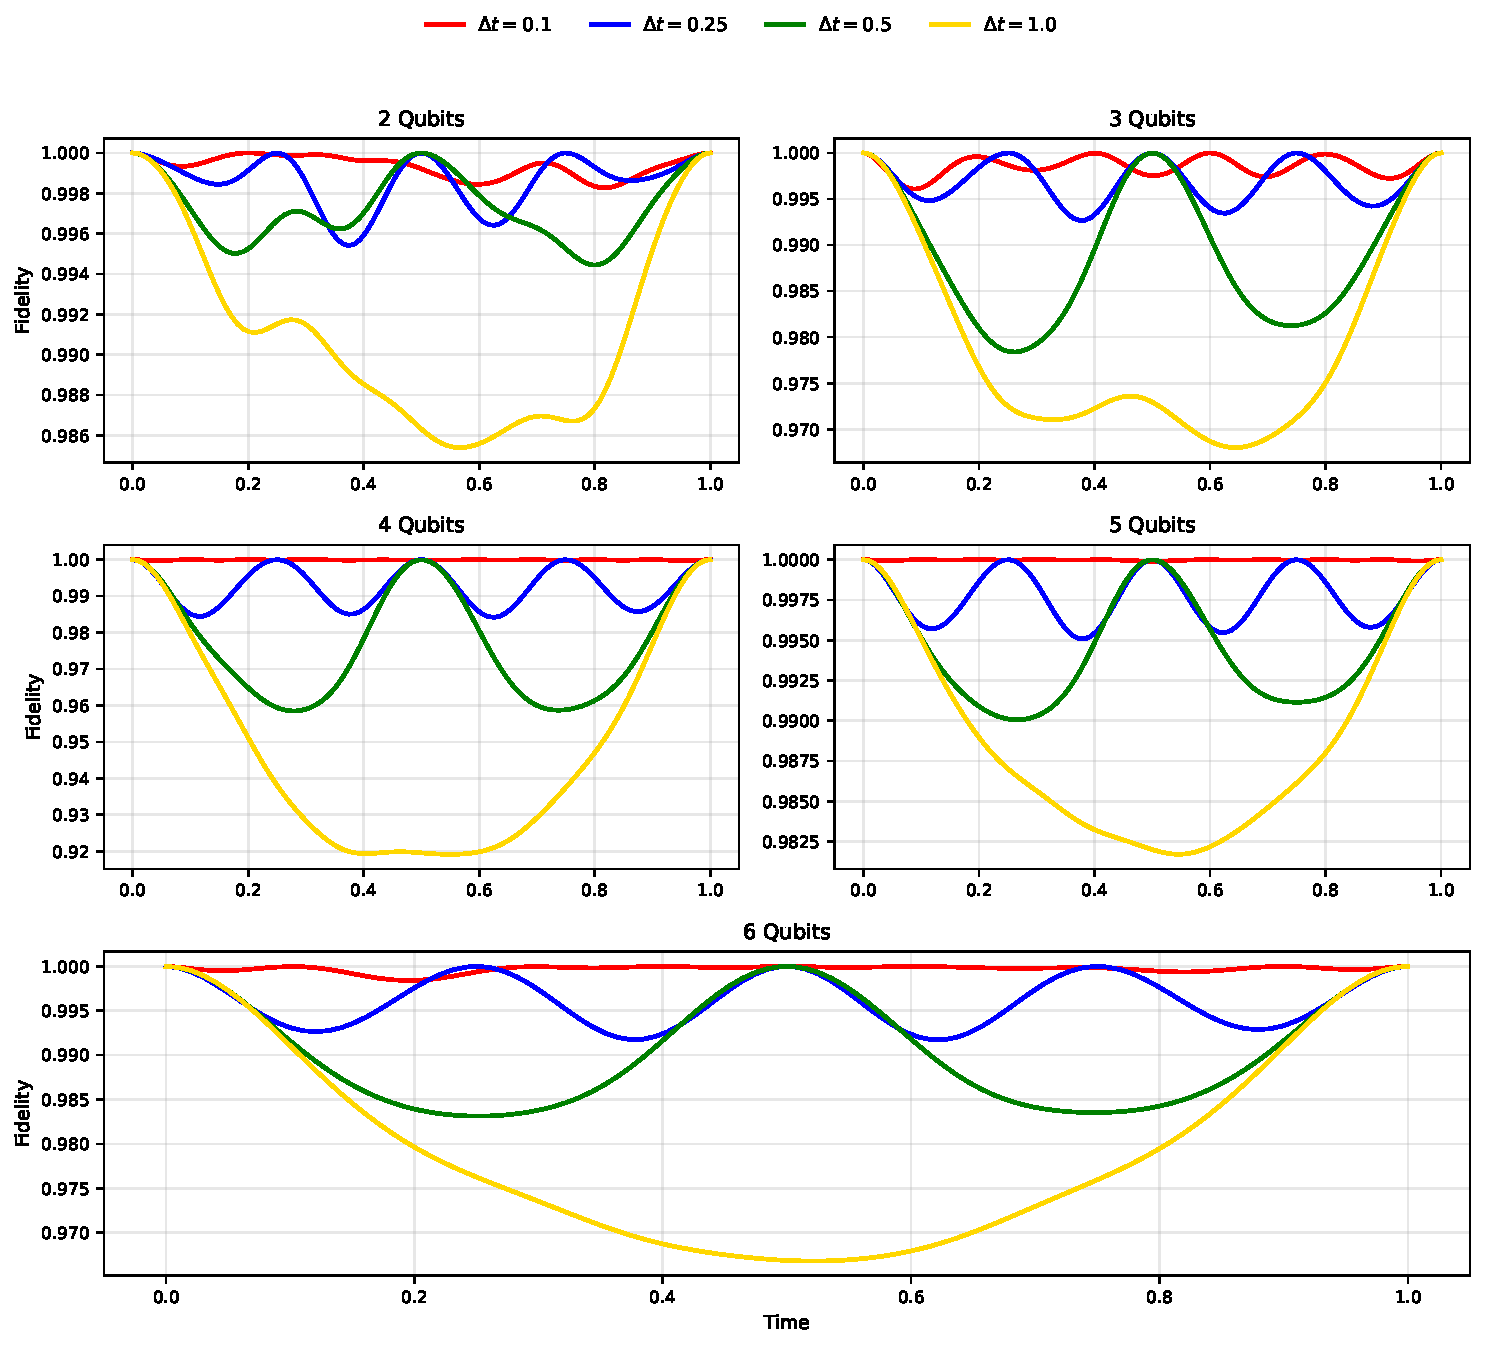
\includegraphics[width=0.8\textwidth]{images/fidelity_qubits_2to6-with.pdf}
  {\small (b)}

  \caption[Fidelity of the predicted unitary evolution for 2- to 6-qubit systems]{Fidelity of the predicted unitary evolution for \textit{model2}--\textit{model6}, shown (a) before and (b) after SVD-based post-processing error correction.}
  \label{fig:res-fid-2to6}
\end{figure}

\begin{figure}[htbp]
  \centering
  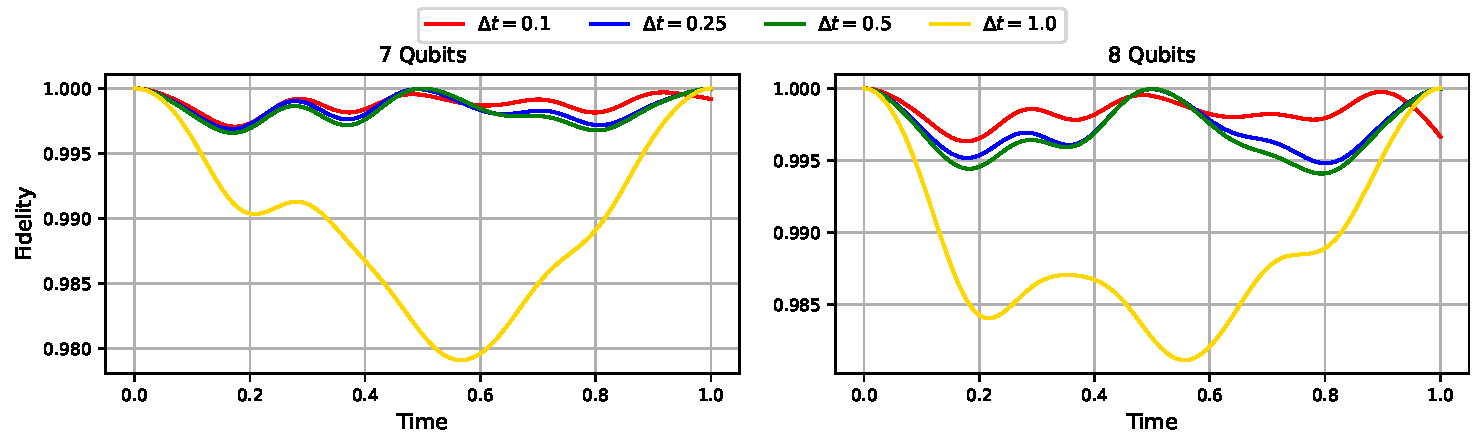
\includegraphics[width=0.99\textwidth]{images/fidelity_qubits_7and8-trotter.pdf}
  {\small (a)}

  \medskip

  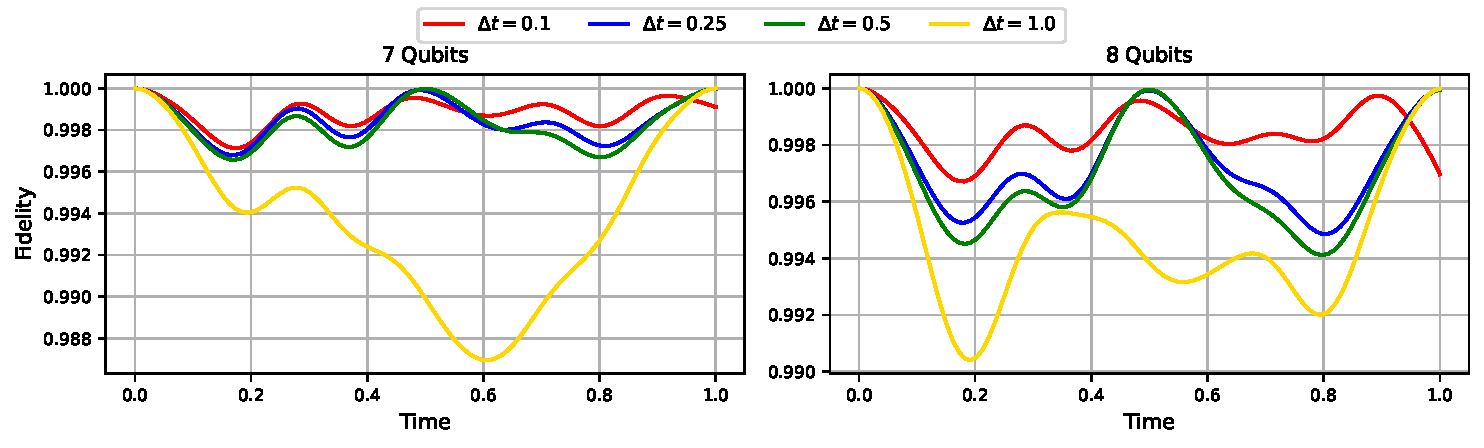
\includegraphics[width=0.99\textwidth]{images/fidelity_qubits_7and8-magnus.pdf}
  {\small (b)}

  \caption[Fidelity performance for 7- and 8-qubit Ising systems]{Fidelity performance for 7- and 8-qubit systems under the four training setups considered for the Ising Hamiltonian system. (a) Trotter-based model. (b) Magnus-based model.}
  \label{fig:res-fid78}
\end{figure}

\begin{figure}[htbp]
  \centering
  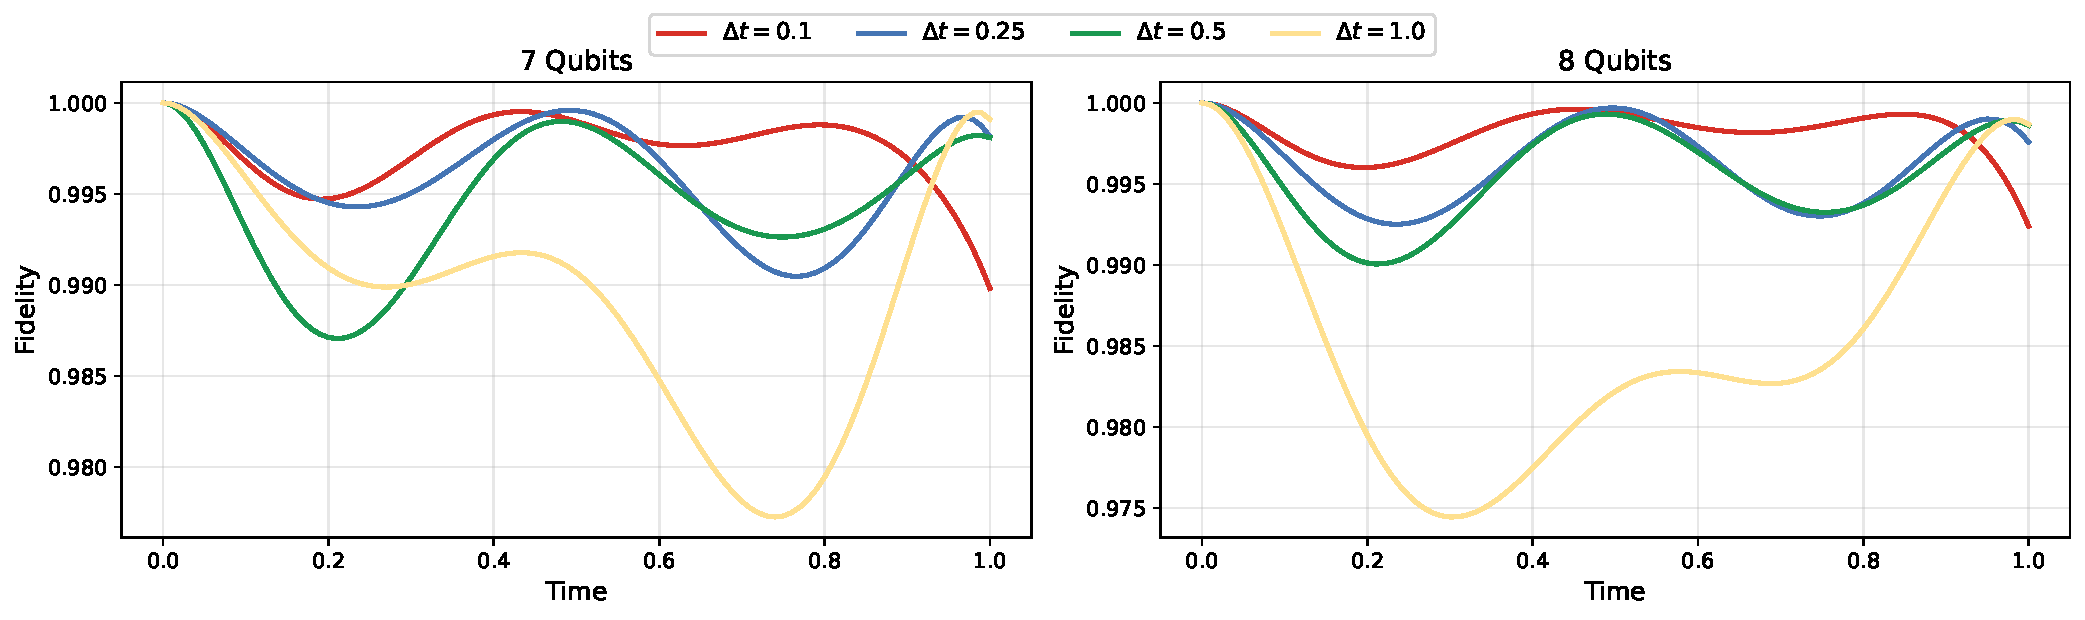
\includegraphics[width=0.99\textwidth]{images/fidelity_xyz_single_trotter.pdf}
  {\small (a)}

  \medskip

  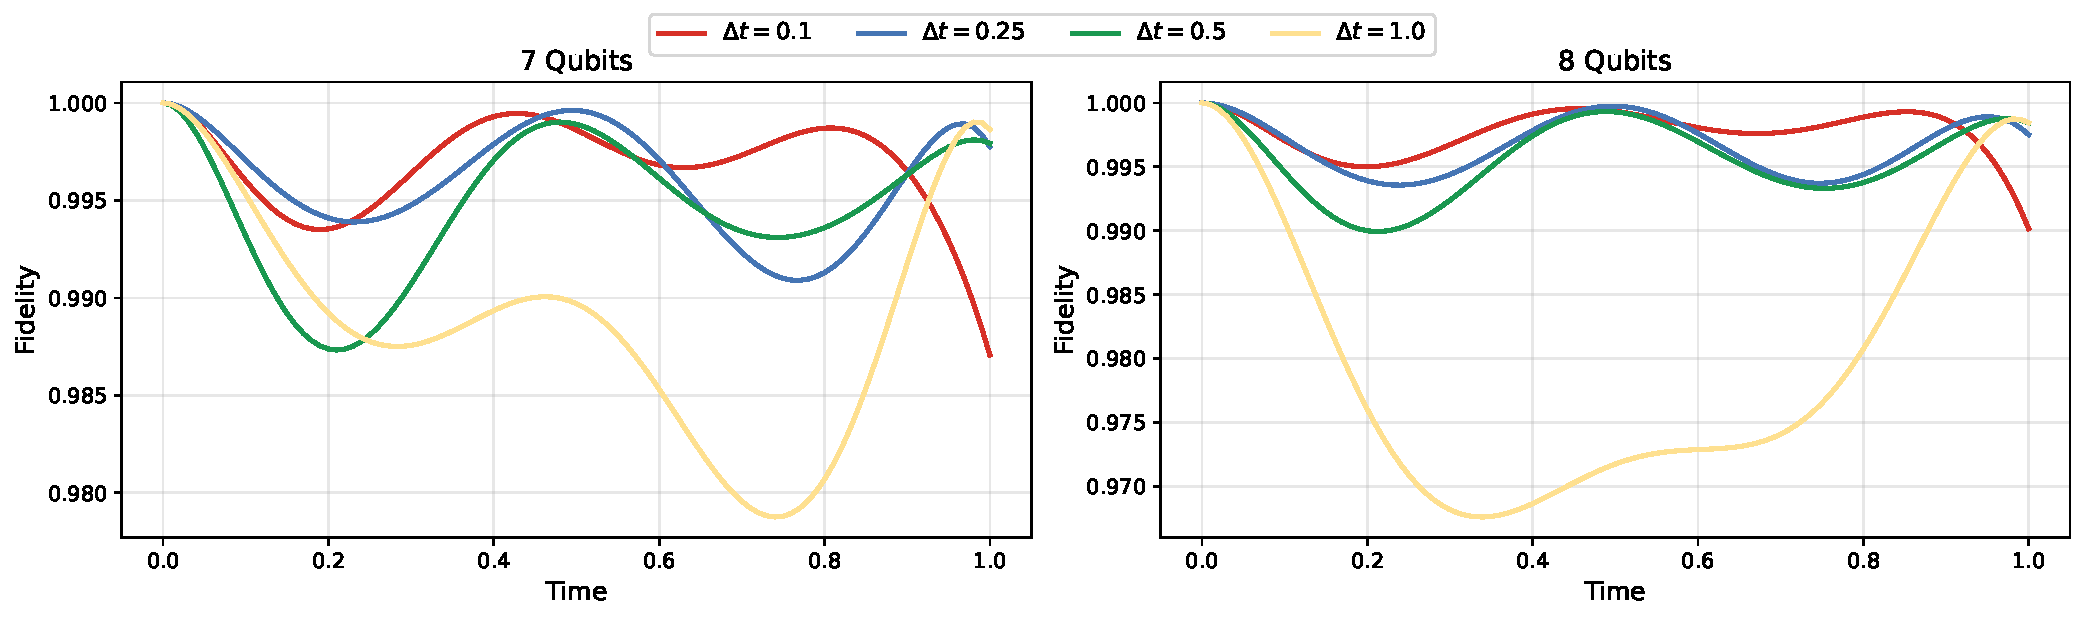
\includegraphics[width=0.99\textwidth]{images/fidelity_xyz_single_magnus.pdf}
  {\small (b)}

  \caption[Fidelity performance for 7- and 8-qubit $XYZ$ systems]{Fidelity performance for 7- and 8-qubit systems under the four training setups considered for the $XYZ$ Hamiltonian system. (a) Trotter-based model. (b) Magnus-based model.}
  \label{fig:res-fid78xyz}
\end{figure}

\subsection{Quantum state dynamics}
\label{sec:res-state-dynamics}

To further validate the model's ability to reproduce quantum state dynamics, we evolve a randomly sampled initial state $\rho_0$ under two distinct time-evolution operators: (i) the exact unitary $U(t)$ computed via the second-order Magnus expansion, and (ii) the unitary $U_\theta(t)$ predicted by the trained model without SVD correction. At each time $t \in [0,1]$, we compute the evolved density matrix according and track the diagonal elements $\rho_{ii}(t)$, which correspond to the occupation probabilities of the computational basis states. Figures~\ref{fig:res-state-dynamics-2to5} and~\ref{fig:res-state-dynamics-6to8} show these populations for systems ranging from 2 to 8 qubits, comparing the model predictions against the exact reference. In all cases, the trajectories are in close agreement, with only minor deviations consistent with the gate fidelity values reported in the preceding section.

\begin{figure}[htbp]
\centering
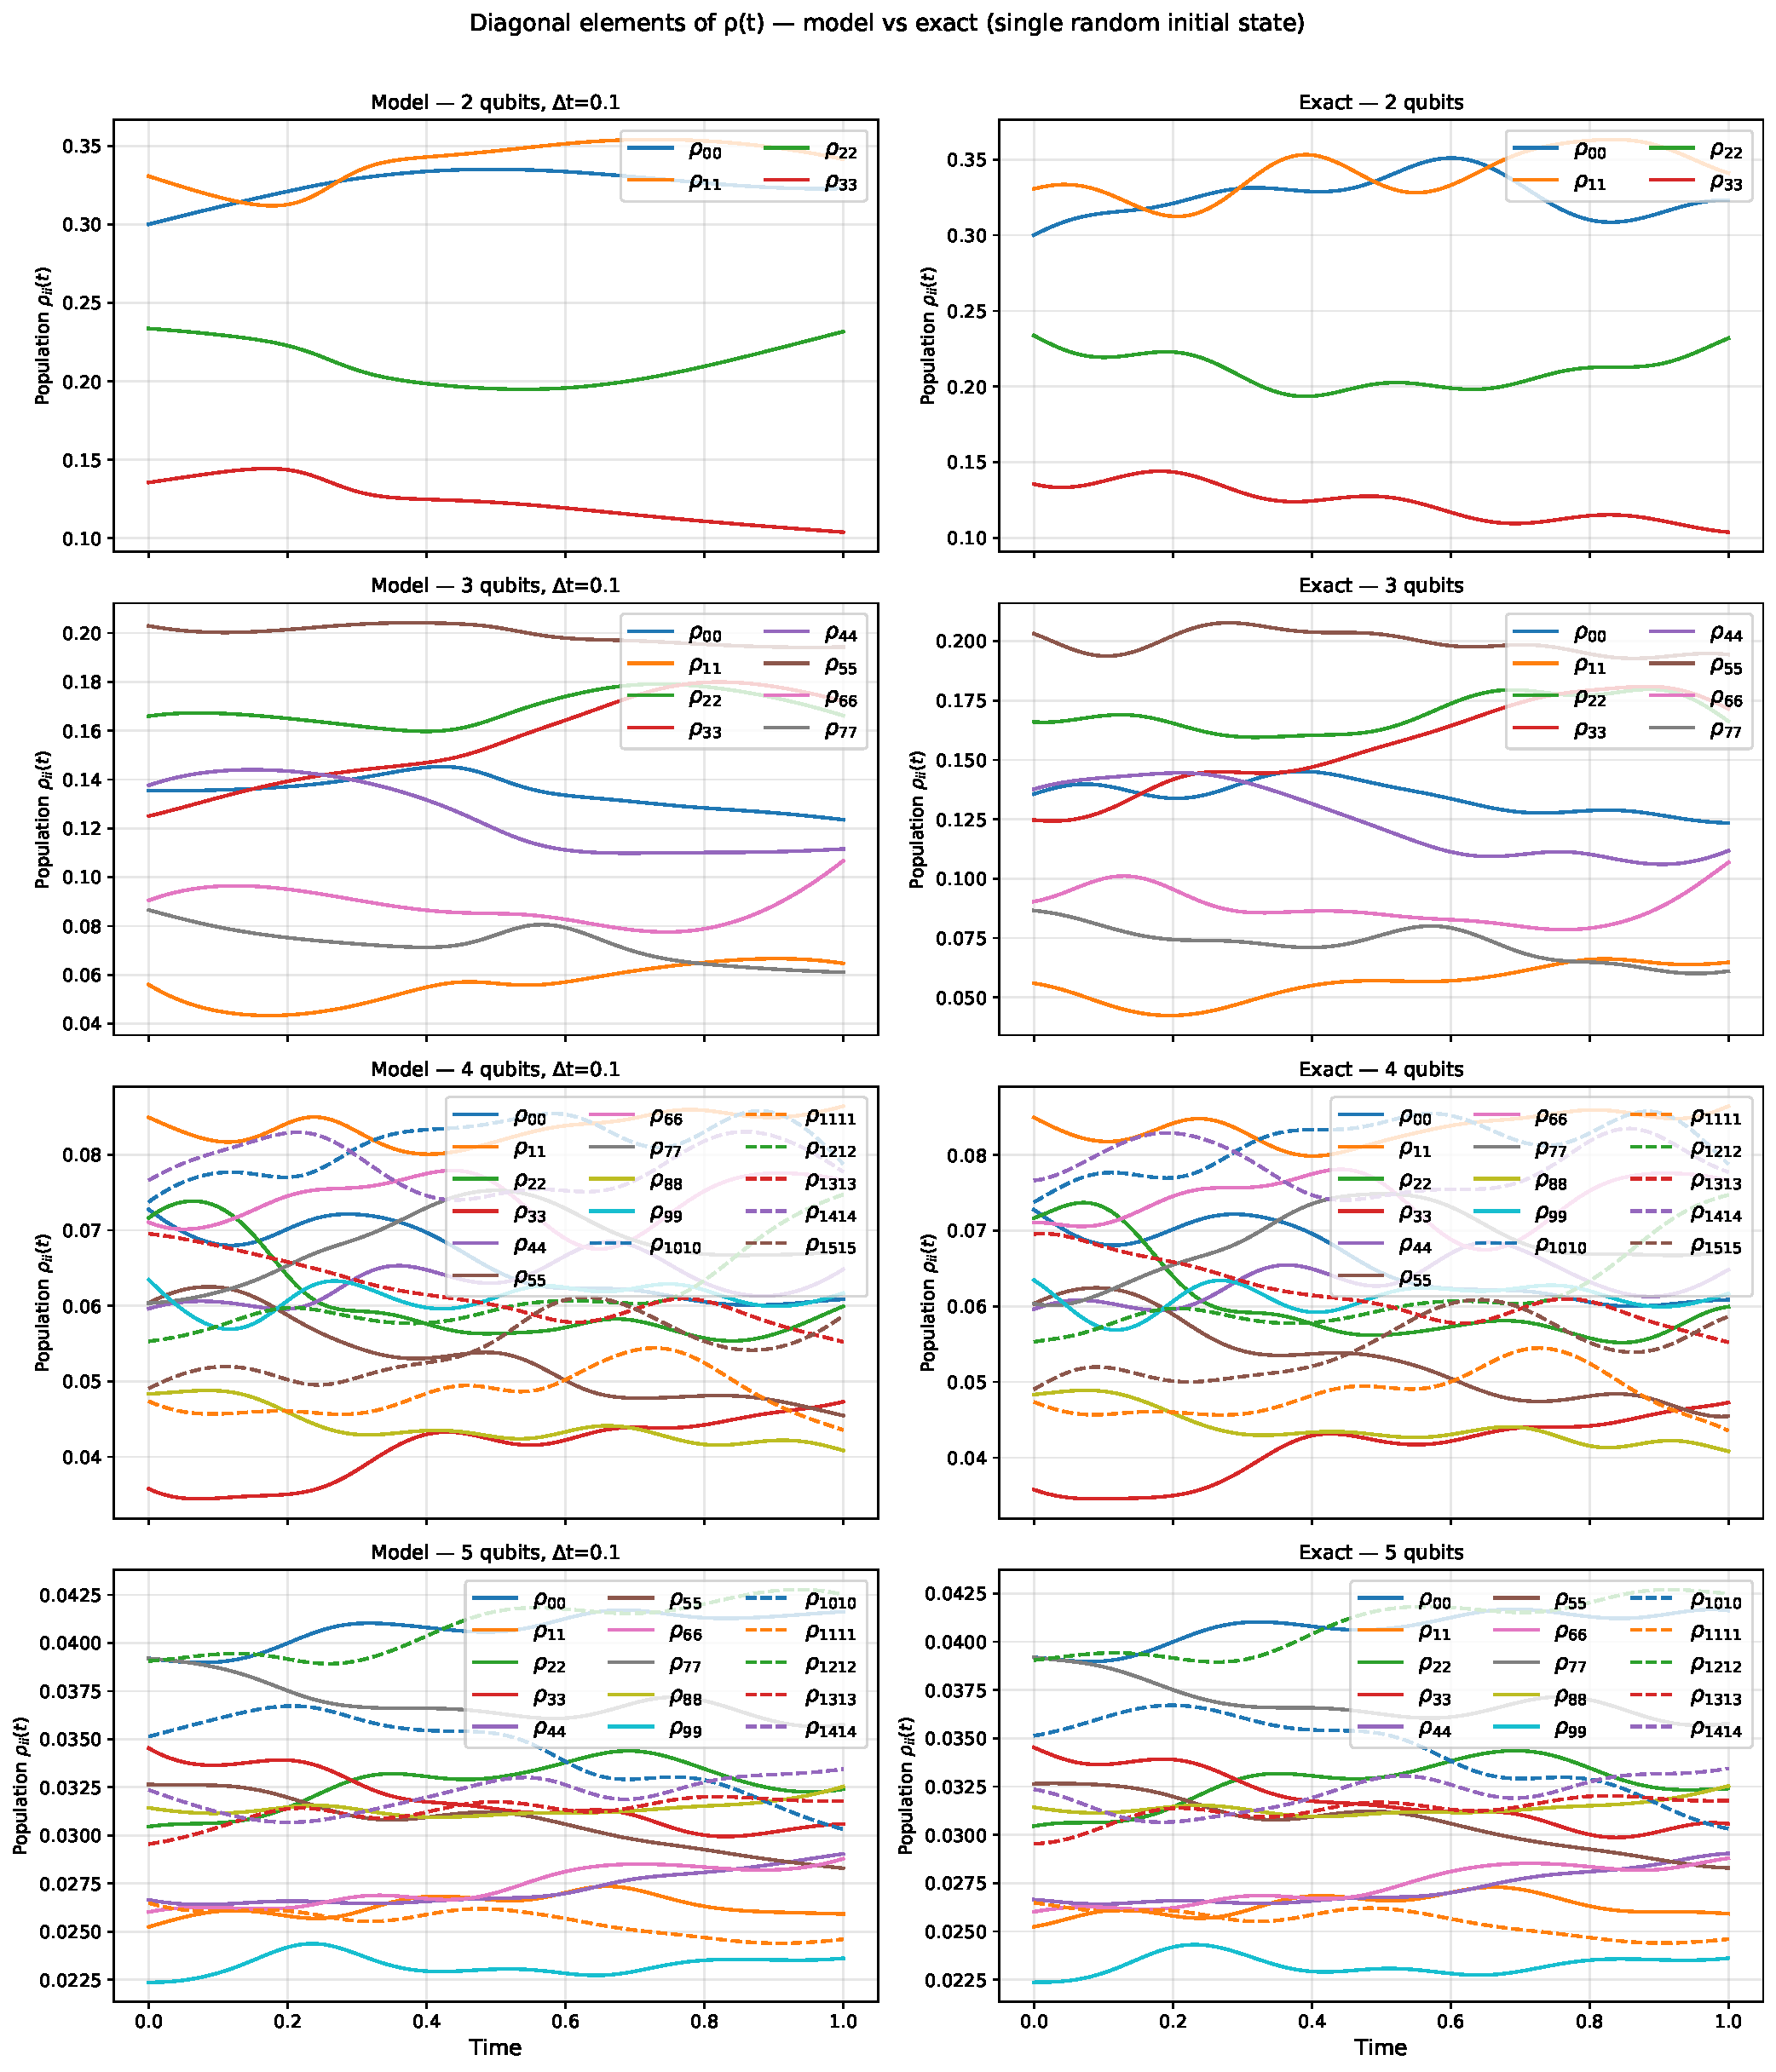
\includegraphics[width=0.99\textwidth]{images/state_dynamics_populations_2to5.pdf}
\caption[Populations of the evolved density matrix for 2- to 5-qubit systems]{Diagonal elements $\rho_{ii}(t)$ of the evolved density matrix for systems of 2 to 5 qubits, comparing the model prediction (left column) against the exact unitary evolution (right column). Each curve corresponds to a different basis state population, for a single randomly sampled initial state $\rho_0$ and training time step $\Delta t = 0.1$. The physical system considered is described by the general Pauli Hamiltonian $H_{\mathrm{general}}(t)$, which includes all possible Pauli components in the $N$-qubit operator basis.}
\label{fig:res-state-dynamics-2to5}
\end{figure}

\begin{figure}[htbp]
\centering
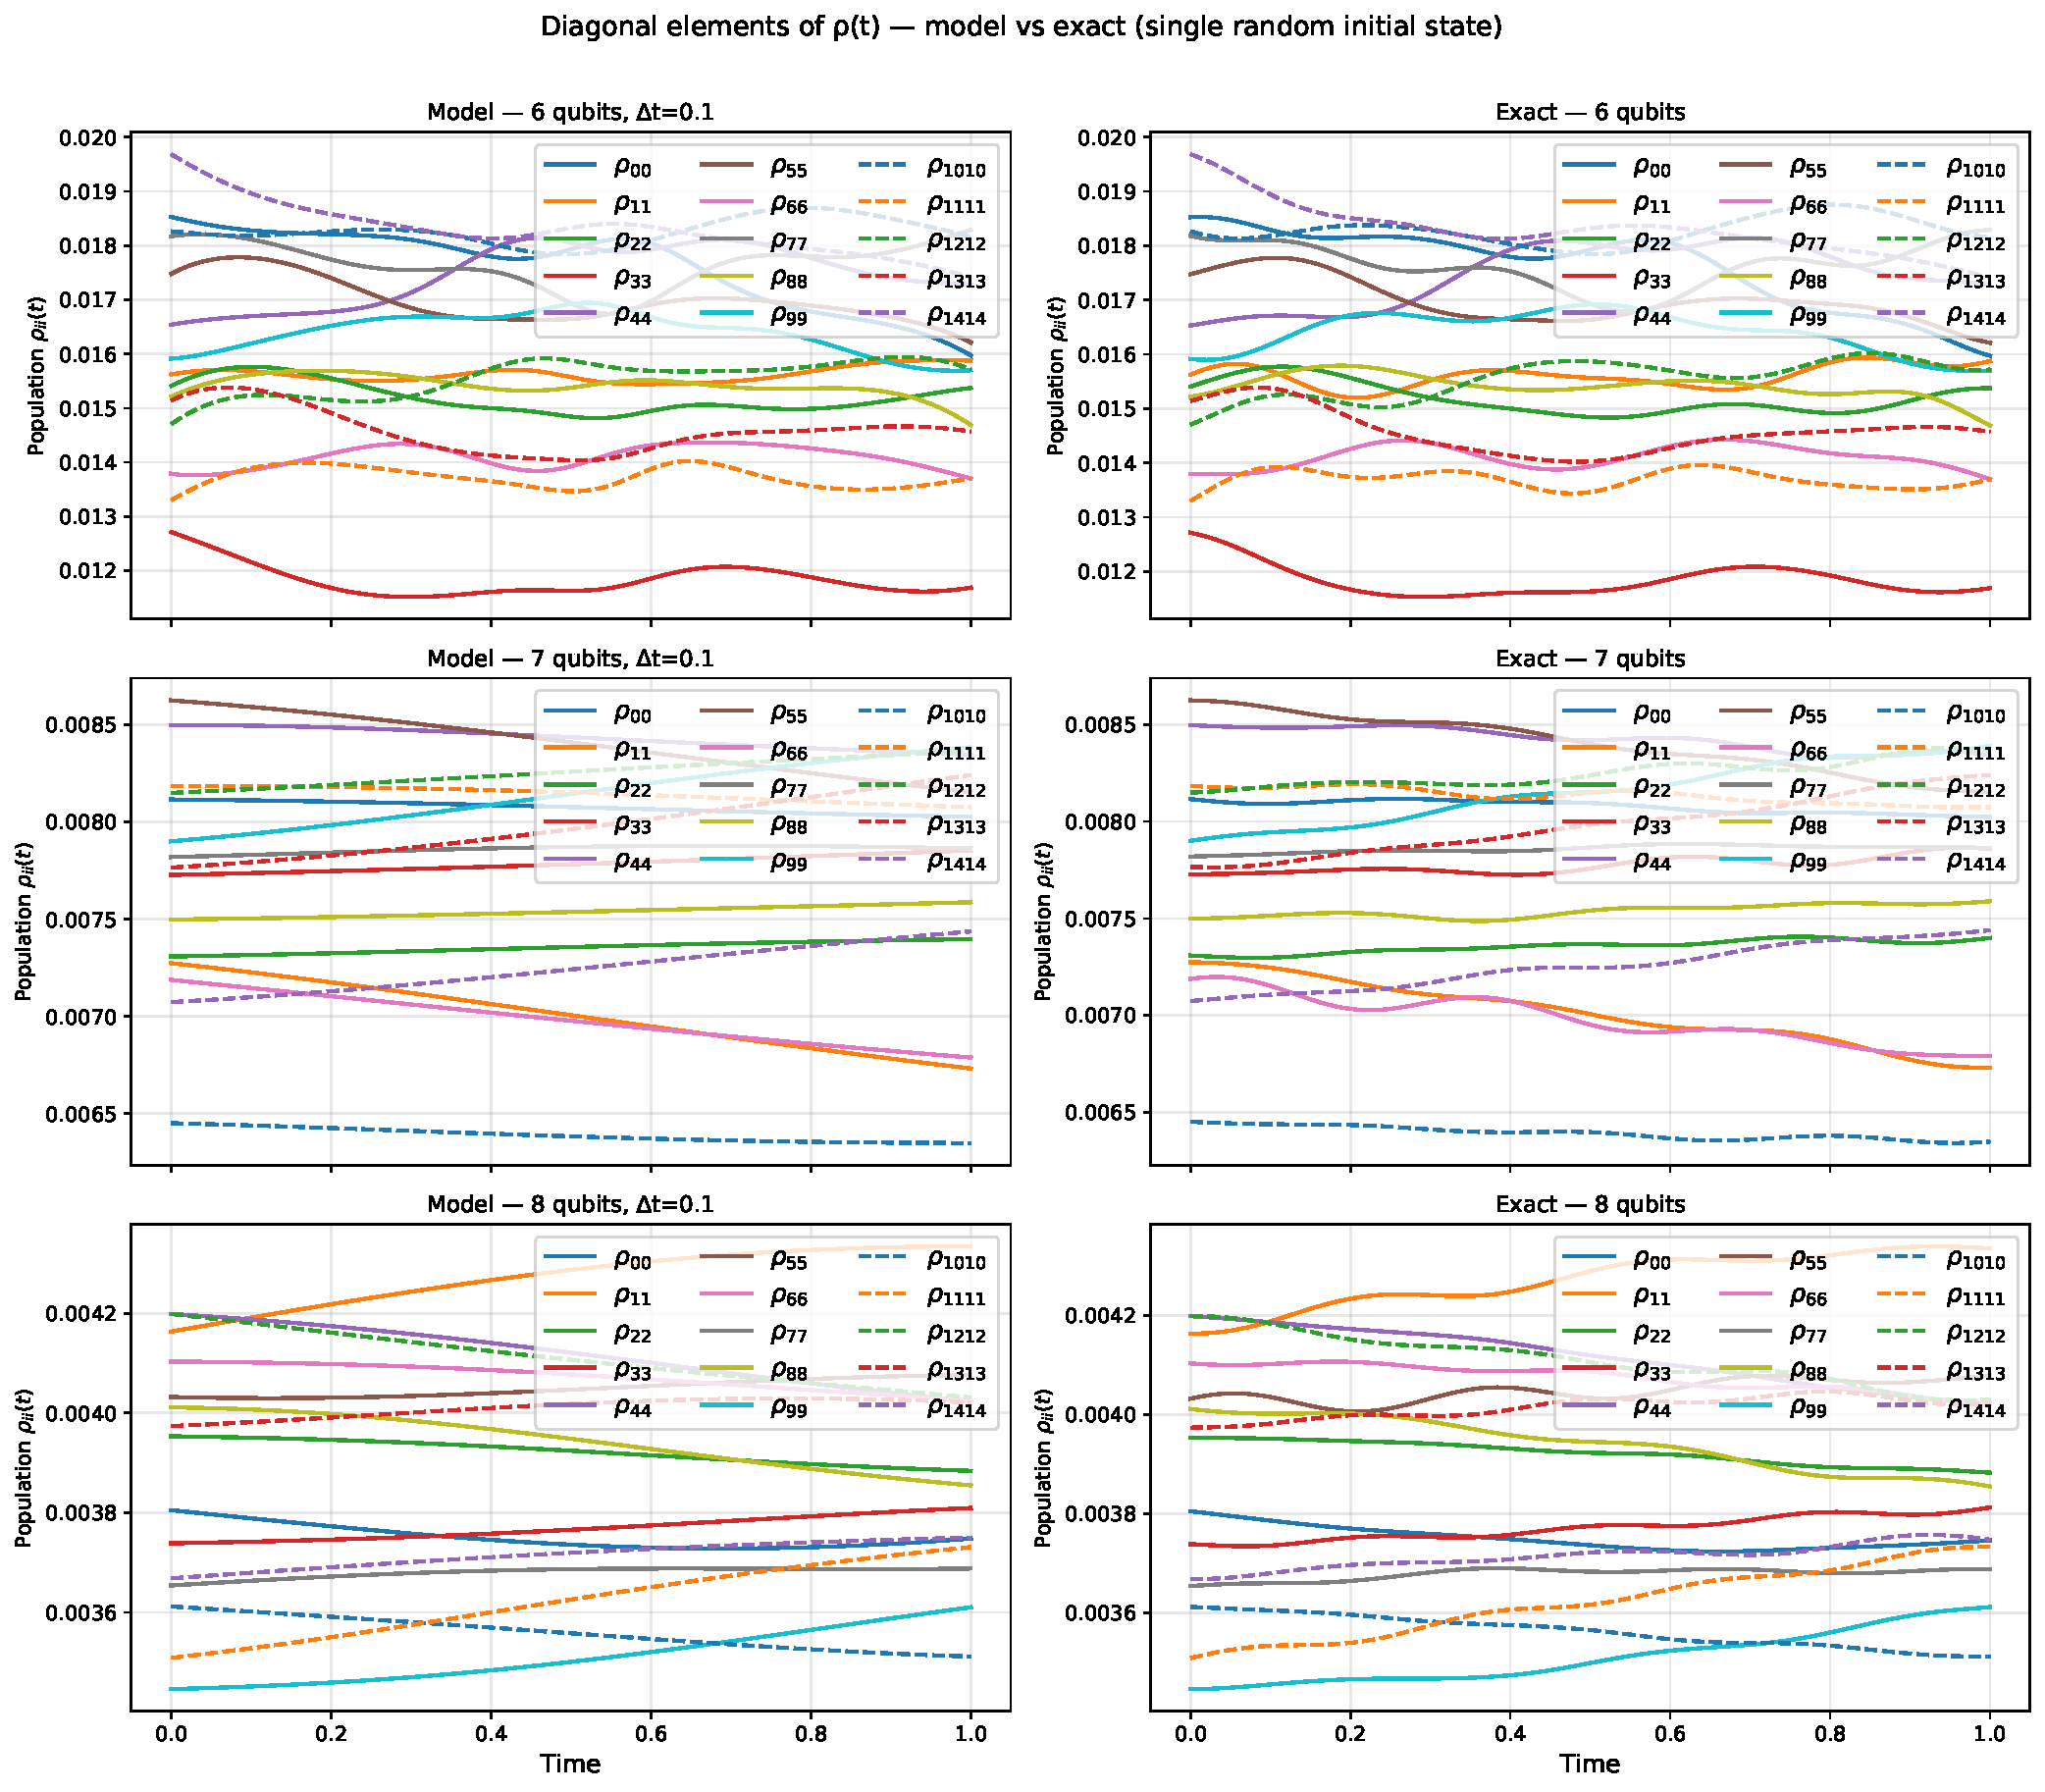
\includegraphics[width=0.99\textwidth]{images/state_dynamics_populations_6to8.pdf}
\caption[Populations of the evolved density matrix for 6- to 8-qubit systems]{Same as Fig.~\ref{fig:res-state-dynamics-2to5} for systems of 6 to 8 qubits. For the 6-qubit case, the physical system is described by the general Pauli Hamiltonian $H_{\mathrm{general}}(t)$. For the 7- and 8-qubit cases, the physical system is described by the nearest-neighbor Ising Hamiltonian $H_{\mathrm{Ising}}(t)$, for which the model predicts the coefficients of an effective Hamiltonian $H_\mathrm{eff}(t)$, from which the unitary is computed via the Magnus expansion.}
\label{fig:res-state-dynamics-6to8}
\end{figure}

\subsection{Statistical analysis}
\label{sec:res-statistics}

To ensure that our evaluation did not rely on a single Hamiltonian realization per system size, we performed an additional statistical analysis to assess the model's robustness in interpolating unitary dynamics across diverse configurations. Three families of Hamiltonians were considered: the general Pauli Hamiltonian with all non-zero components (systems up to 6 qubits), the nearest-neighbor Ising model (7 and 8 qubits), and the nearest-neighbor $XYZ$ Heisenberg model (7 and 8 qubits). For the general Pauli case, we carried out 100 independent training runs per system size. Due to computational resource constraints, this analysis was limited to 50 independent runs for the 7- and 8-qubit Ising Hamiltonian, 50 independent runs for the 7-qubit $XYZ$ Hamiltonian, and 20 independent runs for the 8-qubit $XYZ$ Hamiltonian. In each run, the amplitudes, frequencies, and phases defining the Hamiltonian were independently sampled from uniform distributions according to Section~\ref{sec:res-systems}. This corresponds to $4^N - 1$ independent parameters for systems of up to 6 qubits, $2N - 1$ parameters for the Ising Hamiltonians, and $3(N-1)$ parameters for the $XYZ$ Hamiltonians. These parameters were used to construct the target unitary evolutions, generate the corresponding training datasets, and train the model under identical conditions. Applying the same fidelity-evaluation pipeline yielded a collection of fidelity curves $F^{(k)}(t)$, with $k = 1, \ldots, N_r$, where $N_r$ is the number of independent runs for each system size and Hamiltonian family. Each curve is obtained by evaluating the gate fidelity of Eq.~\eqref{eq:res-metric-fidelity} on a uniform grid of 100 points in $t \in [0,1]$, comparing the model prediction against the numerically computed target unitary. The mean fidelity $F_{\mu}(t)$ and the fidelity standard deviation $F_{\sigma}(t)$ were computed as
\begin{align}
  F_{\mu}(t) &= \frac{1}{N_r} \sum_{k=1}^{N_r} F^{(k)}(t), \\
  F_{\sigma}(t) &= \sqrt{ \frac{1}{N_r-1} \sum_{k=1}^{N_r} \qty( F^{(k)}(t) - F_{\mu}(t) )^2 },
\end{align}
where $F^{(k)}(t)$ is the gate fidelity of the $k$-th run at time $t$.

Figures~\ref{fig:res-stat-2to6}, \ref{fig:res-stat-78-ising}, and \ref{fig:res-stat-78-xyz} summarize the mean fidelity and standard deviation across all independent runs, providing a quantitative assessment of the variability in the model's performance. For each system size up to 6 qubits, two panels are shown: the first compares the raw model outputs with the target unitary evolutions, while the second reports the nearest-unitary matrices obtained through SVD-based post-processing. For 7- and 8-qubit systems, because unitarity is guaranteed by the Trotterization or Magnus expansion, SVD corrections are not required. Since these results closely match those obtained in the single-training analysis, we expect a similar statistical behavior for other values of $\Delta t$ when applying the same procedure.

Across all analyses, the standard deviation remains consistently low. Even without enforcing unitarity via SVD, the variability is small, and after error correction the associated uncertainty becomes negligible to the point that it is not visually distinguishable in the figure. Moreover, no specific regions were identified where the model failed to interpolate successfully.

\begin{figure}[htbp]
  \centering
  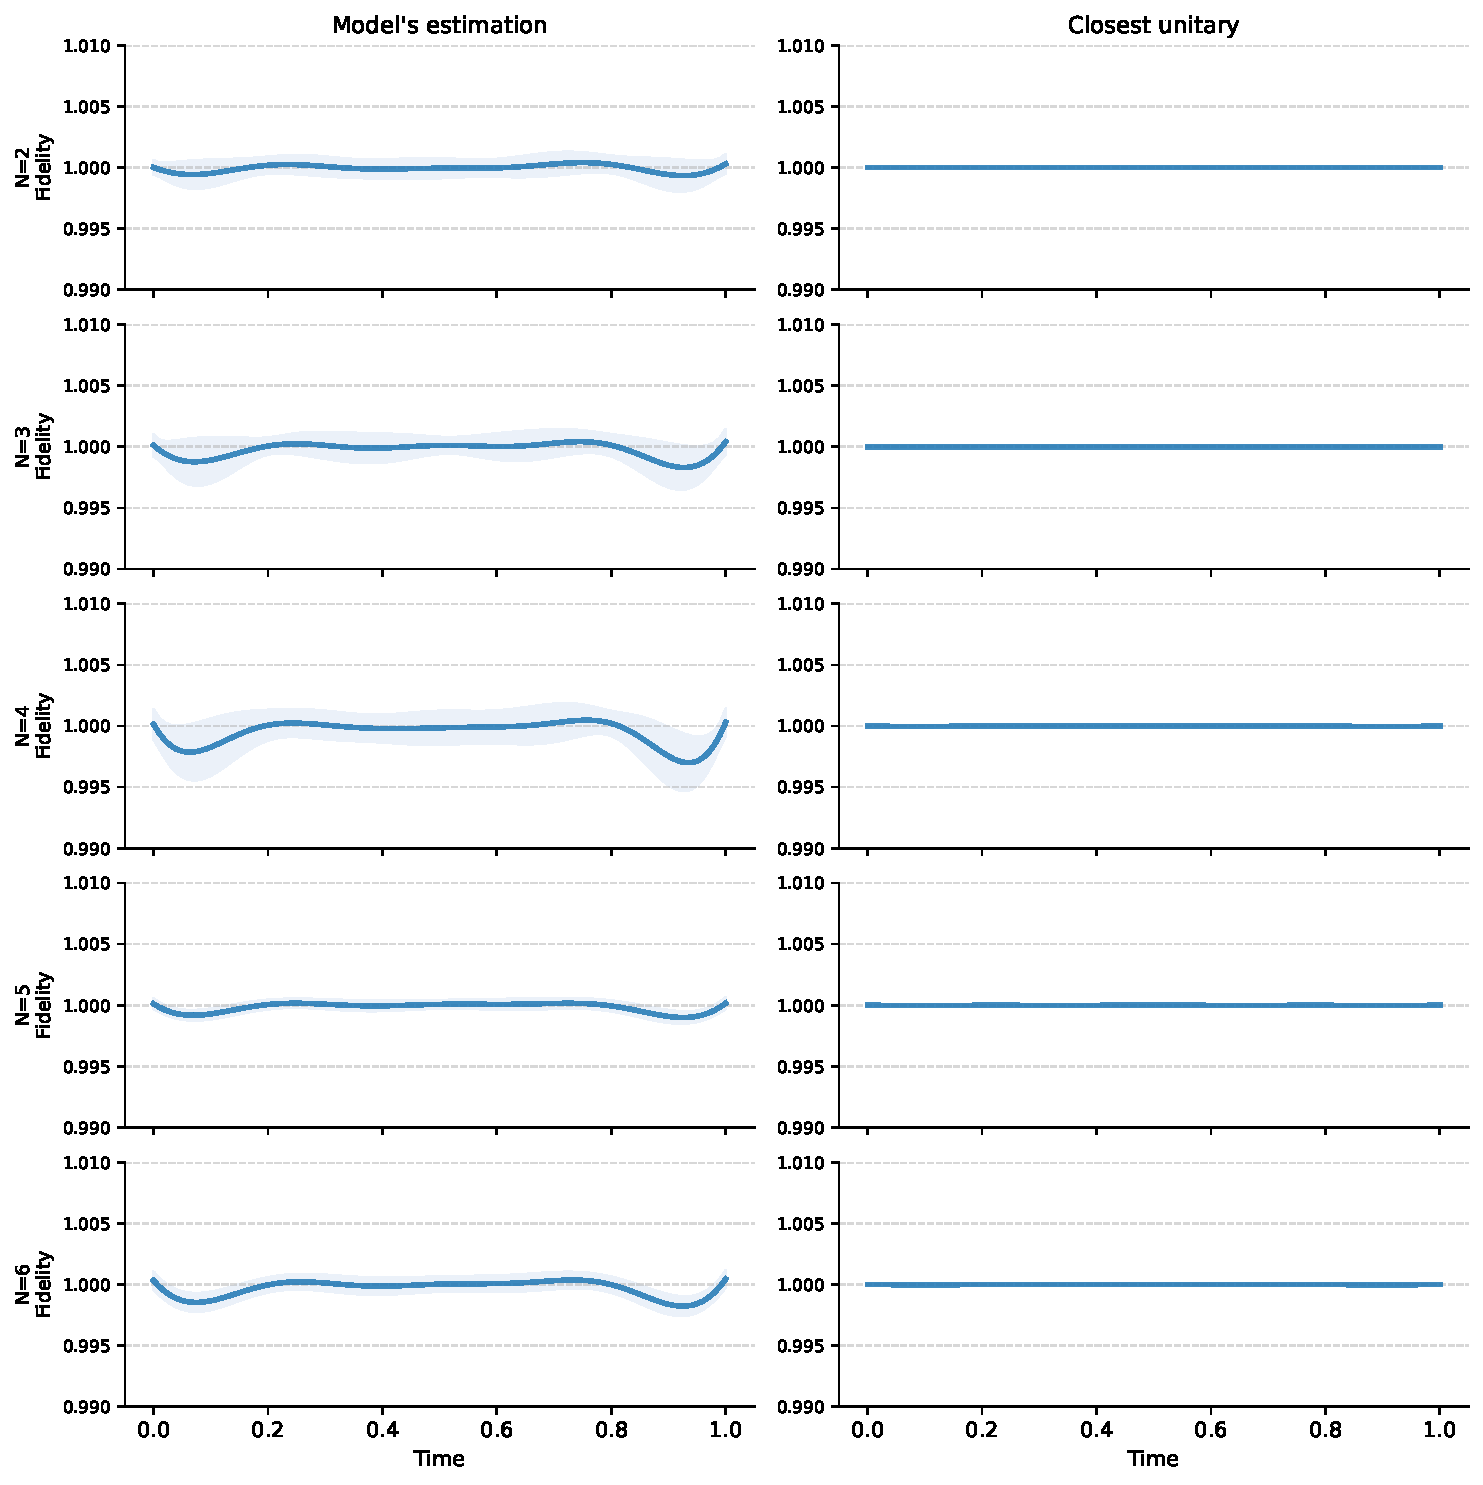
\includegraphics[width=0.99\linewidth]{images/fidelity_statistic_plots_2to6.pdf}
  \caption[Mean fidelity and standard deviation for systems up to 6 qubits]{Mean fidelity and standard deviation across 100 independent training runs for systems up to 6 qubits. Left: raw model output vs.\ target unitary. Right: SVD-corrected output vs.\ target unitary.}
  \label{fig:res-stat-2to6}
\end{figure}

\begin{figure}[htbp]
  \centering
  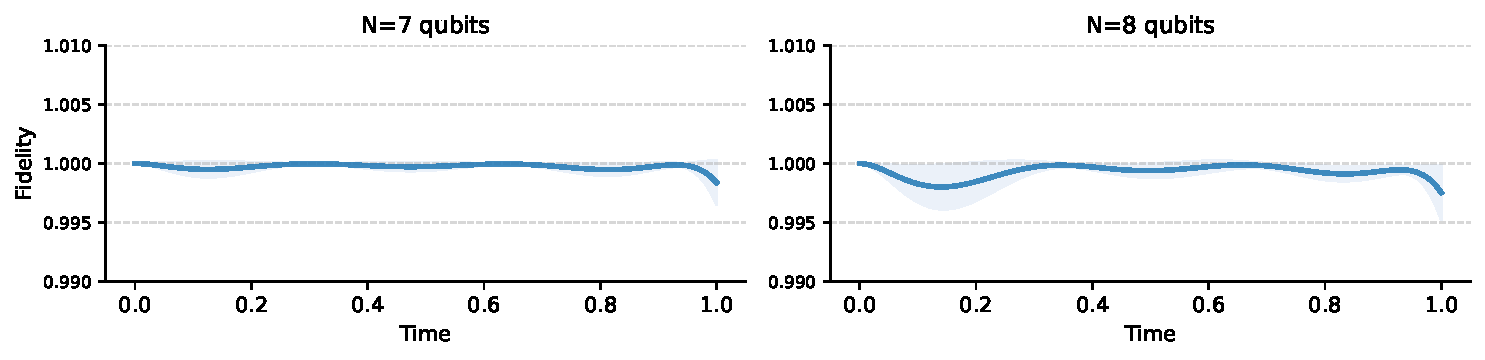
\includegraphics[width=0.99\linewidth]{images/fidelity_statistic_plots_7to8.pdf}
  \caption[Mean fidelity and standard deviation for 7- and 8-qubit Ising systems]{Same as Fig.~\ref{fig:res-stat-2to6} for 7- and 8-qubit systems under the nearest-neighbor Ising Hamiltonian (50 independent runs).}
  \label{fig:res-stat-78-ising}
\end{figure}

\begin{figure}[htbp]
  \centering
  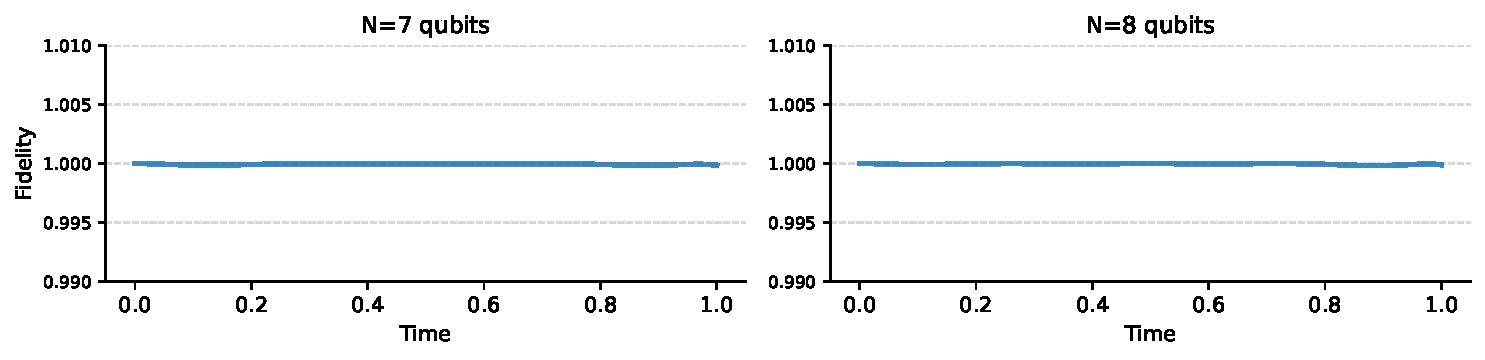
\includegraphics[width=0.99\linewidth]{images/fidelity_xyz_N7_to_N8.pdf}
  \caption[Mean fidelity and standard deviation for 7- and 8-qubit $XYZ$ systems]{Same as Fig.~\ref{fig:res-stat-2to6} for 7- and 8-qubit systems under the nearest-neighbor $XYZ$ Heisenberg Hamiltonian (50 runs for 7 qubits, 20 runs for 8 qubits).}
  \label{fig:res-stat-78-xyz}
\end{figure}

\subsection{Trace-distance analysis}
\label{sec:res-trace-distance}

To extend our statistical analyses, we employ the trace distance as an additional figure of merit. For two density matrices $\rho$ and $\sigma$, the trace distance is defined as
\begin{equation}
\label{eq:res-trace-distance}
T(\rho, \sigma) = \frac{1}{2} \norm{ \rho - \sigma }_1 = \frac{1}{2} \sum_i |\lambda_i|,
\end{equation}
where $\lambda_i$ are the eigenvalues of the Hermitian operator $\rho - \sigma$, and $T \in [0,1]$. Following the same procedure as in the statistical analysis above, we evaluate the trace distance between the states evolved under the predicted and exact unitaries over an ensemble of $N_s = 50$ random initial states, on a uniform grid of $N_t = 100$ points in $t \in [0,1]$. The initial states are sampled from the Hilbert--Schmidt measure, as described in Section~\ref{sec:res-loss-function}.

For each qubit size, we compute the trace distances
\begin{equation}
  T_i(t) = T\qty(\rho_i(t),\sigma_i(t)),
\end{equation}
where $\rho_i(t) = U_{\theta_{\mathrm{opt}}}(t)\, \rho_0^i\, U_{\theta_{\mathrm{opt}}}^{\dagger}(t)$ and $\sigma_i(t) = U(t)\, \rho_0^i\, U^{\dagger}(t)$ are the states evolved under the predicted and exact unitaries respectively, and $i=1,\ldots,N_s$ labels the random initial states. The reported value corresponds to the mean trace distance,
\begin{equation}
  T_{\mu}(t)= \frac{1}{N_s} \sum_{i=1}^{N_s} T_{i}(t),
\end{equation}
while the error bars indicate one standard deviation,
\begin{equation}
  T_{\sigma}(t) = \sqrt{ \frac{1}{N_s-1} \sum_{i=1}^{N_s} \qty[T_{i}(t)-T_{\mu}(t)]^2 }.
\end{equation}

Figure~\ref{fig:res-trace-distance} summarizes the trace-distance statistics for models trained using a dataset with $\Delta t = 0.1$. The obtained values remain consistently of the order of $\mathcal{O}(10^{-2})$ across all qubit sizes, indicating a high degree of agreement between the states evolved under the predicted and exact dynamics. This result is particularly significant given that the trace distance is bounded in the interval $[0,1]$ and vanishes if and only if $\rho=\sigma$.

It is also worth noting that all panels in Fig.~\ref{fig:res-trace-distance} include a shaded region representing one standard deviation around the ensemble-averaged trace distance. For system sizes of 6 qubits and larger, the variability becomes sufficiently small that the shaded region is barely visible at the scale of the plots. Taken together, the results presented in this section show that the proposed models achieve both high average fidelity and low state-reconstruction error across the considered range of system sizes, highlighting their ability to accurately infer the underlying quantum dynamics.

\begin{figure}[htbp]
\centering
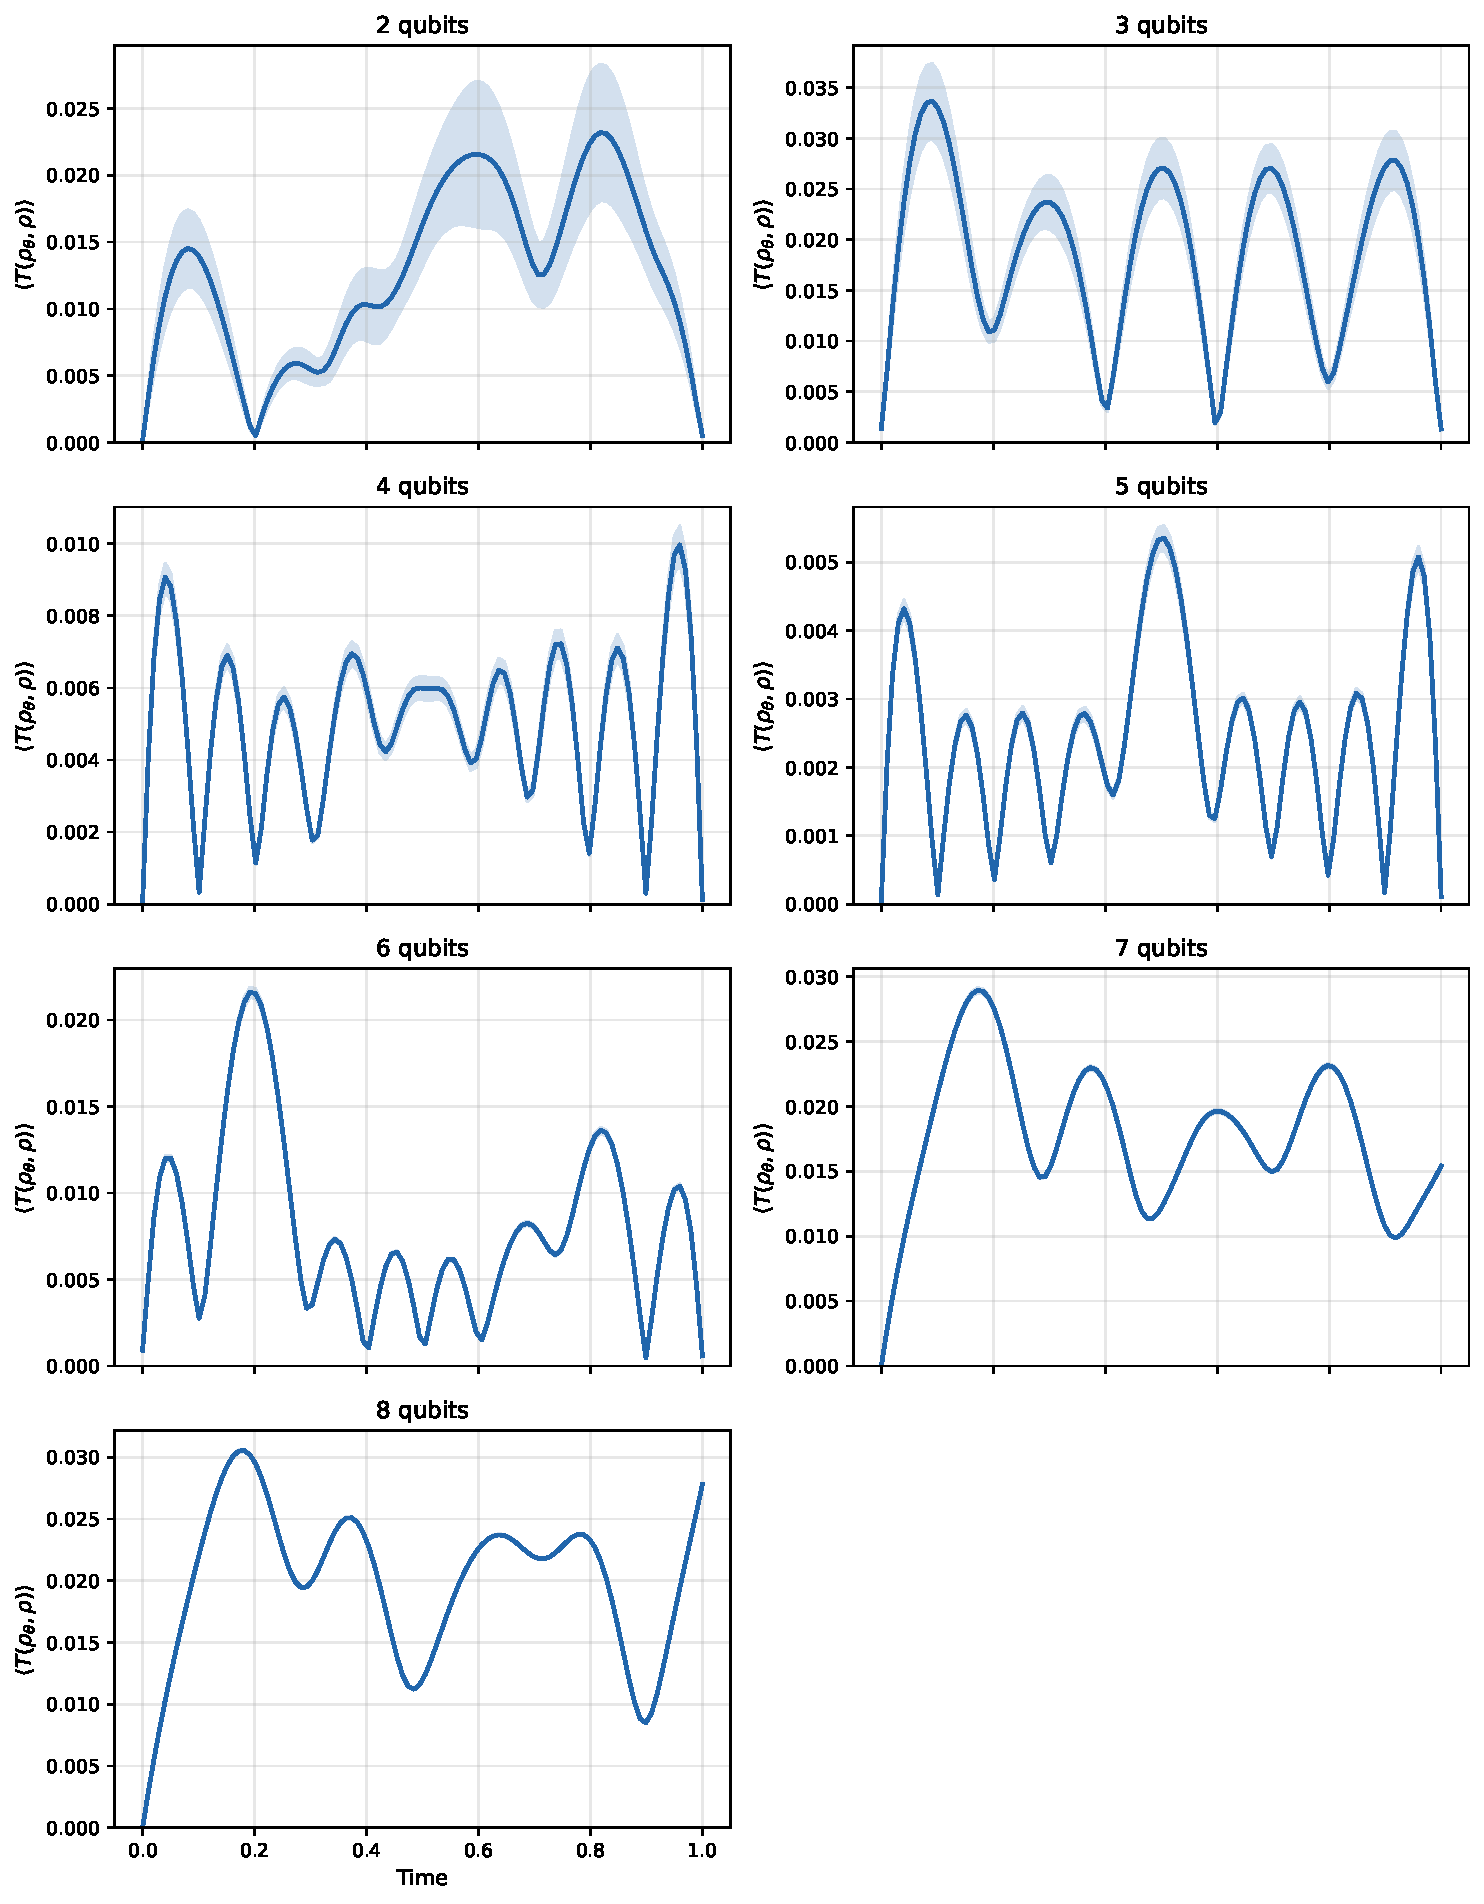
\includegraphics[width=0.99\textwidth]{images/trace_distance_all_N.pdf}
\caption[Mean trace distance between exact and predicted evolutions]{Mean trace distance between states evolved under the exact and predicted unitary operators for system sizes ranging from 2 to 8 qubits. The solid line shows the ensemble average over $N_s=50$ random initial states at each time point, while the shaded region indicates one standard deviation. Trace distances remain of the order of $10^{-2}$ throughout the evolution, demonstrating the accuracy of the learned dynamics.}
\label{fig:res-trace-distance}
\end{figure}

\subsection{Effect of the unitarity imposition term}
\label{sec:res-unitarity-term}

In Section~\ref{sec:res-loss-function}, we introduced the loss function employed during training together with a brief description of each contribution and its physical interpretation. The first two terms naturally incorporate the available knowledge of the system through supervised data constraints. In contrast, the third term introduces an additional soft constraint associated with the unitarity properties of the time-evolution operator, which may not always play a dominant role during the learning process.

Figures~\ref{fig:res-unitarity-1} and~\ref{fig:res-unitarity-2} present a statistical analysis of the impact of including or excluding the unitarity penalty term during training. The analysis was carried out through 25 independent training runs per system size, each considering a distinct realization of the fully non-zero Pauli Hamiltonian, with parameters sampled as described in Section~\ref{sec:res-systems}. As in the preceding analyses, four values of the time grid were considered, $\Delta t \in \{0.1, 0.25, 0.5, 1.0\}$.

The figures compare the mean gate fidelity and its associated standard deviation across multiple independent realizations. The results show that the inclusion of the unitarity term becomes increasingly relevant as the amount of available training data decreases. In particular, for cases with sufficiently dense temporal sampling, such as $\Delta t = 0.1$, both approaches achieve fidelities close to unity over the entire time interval, indicating that the additional unitarity constraint does not provide improvements for the model. For $\Delta t = 0.25$, a small but still noticeable improvement can already be observed when the unitarity term is included.

However, for cases with more limited information, namely $\Delta t = 0.5$ and $\Delta t = 1.0$, the inclusion of the unitarity term significantly improves the overall performance of the model. In these regimes, the additional constraint not only increases the mean fidelity but also reduces the variance across independent realizations, leading to more stable and reliable predictions. This behavior is physically reasonable since, under reduced data availability, one of the few pieces of prior information that remains known with certainty is the unitary nature of the time-evolution operator. Consequently, these results highlight the importance of incorporating physically motivated constraints into the loss function, particularly in low-data regimes.

\begin{figure}[htbp]
\centering

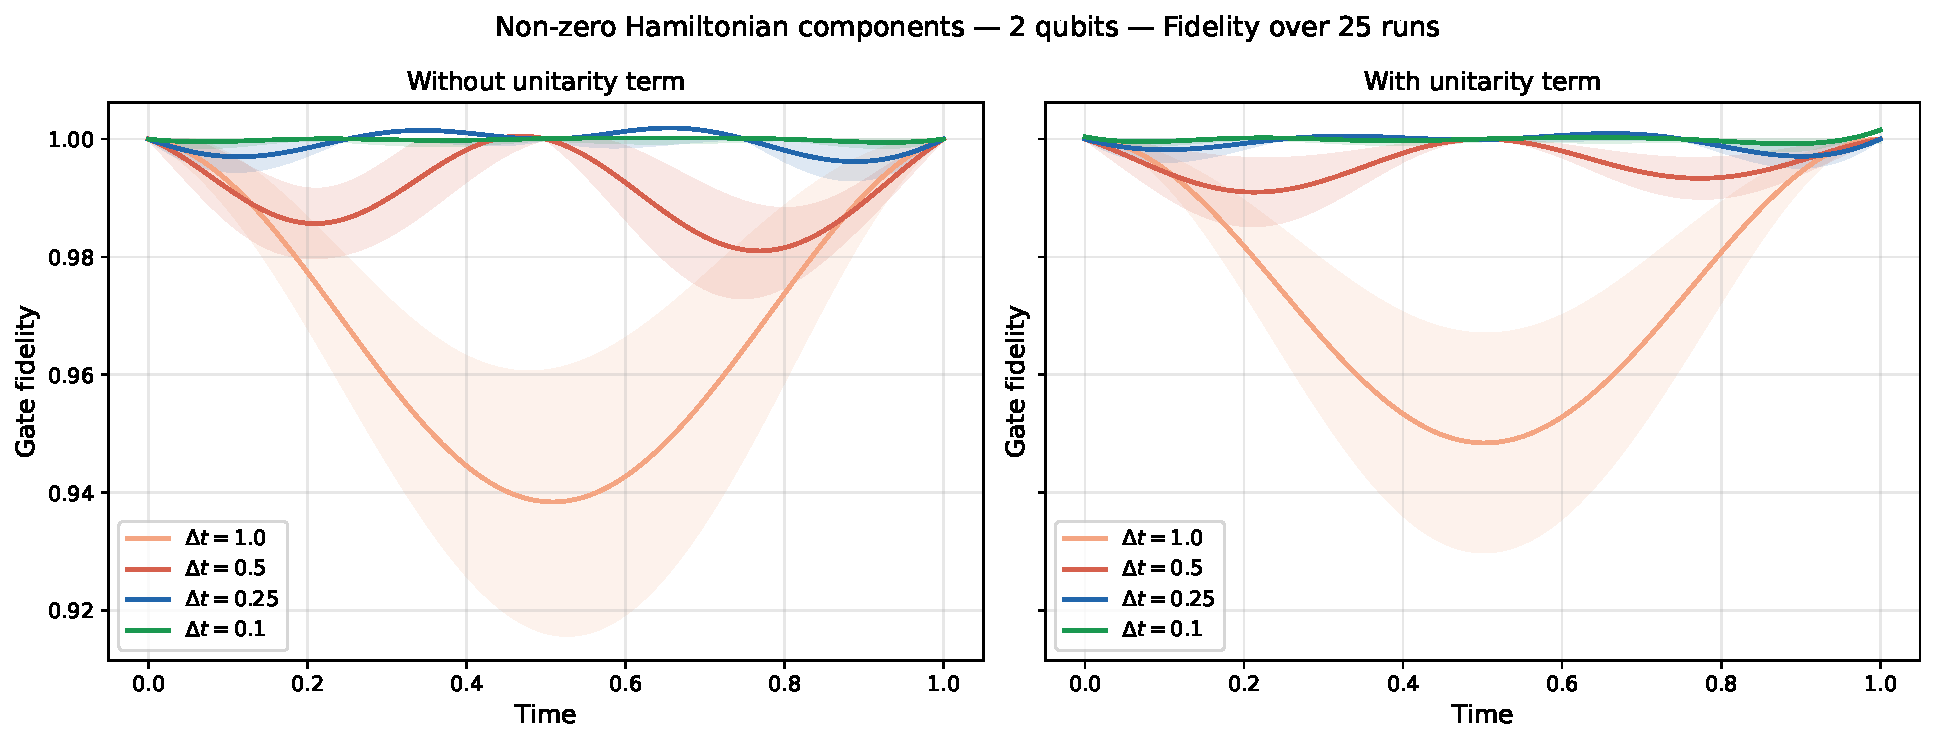
\includegraphics[width=0.88\textwidth]{images/fidelity_unitarity_N2.pdf}
\smallskip
{\small (a) Statistical analysis for the $N=2$ qubit case.}
\medskip

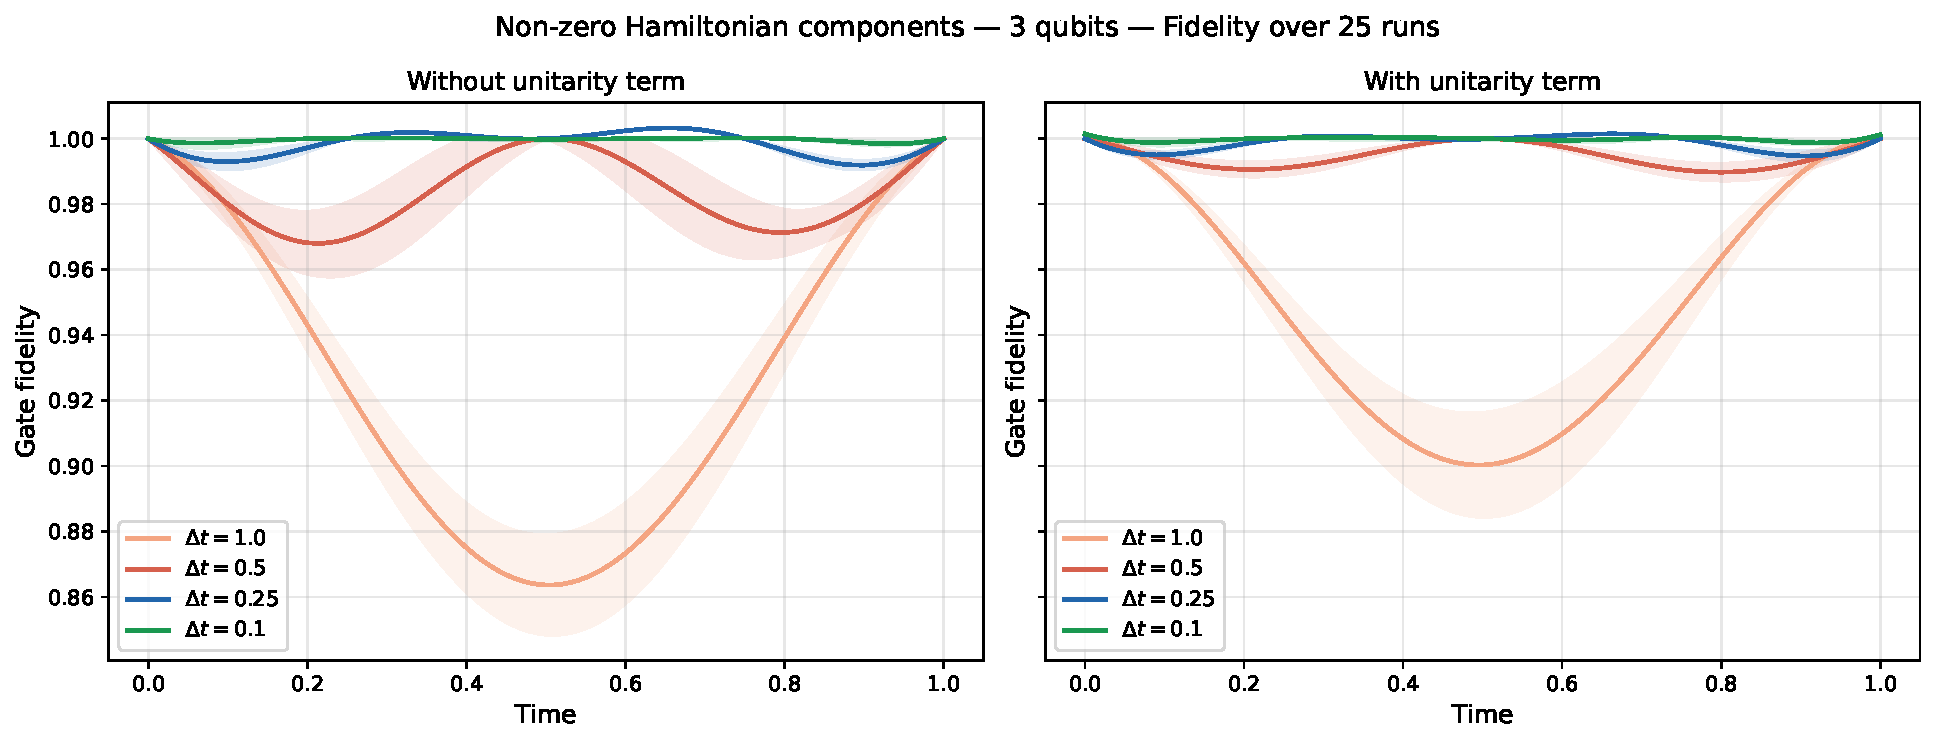
\includegraphics[width=0.88\textwidth]{images/fidelity_unitarity_N3.pdf}
\smallskip
{\small (b) Statistical analysis for the $N=3$ qubit case.}

\caption[Effect of the unitarity term in the loss function ($N=2,3$)]{Statistical analysis of the effect of the unitarity imposition term in the loss function over 25 independent runs for different qubit system sizes. In each figure, the left panel shows the results obtained without the unitarity term, while the right panel includes the additional soft constraint associated with the unitary behavior of the time-evolution operator. Each curve represents the mean gate fidelity as a function of time for different temporal resolutions $\Delta t = 0.1, 0.25, 0.5,$ and $1.0$, while the shaded regions indicate the corresponding standard deviation across independent realizations with randomly generated Hamiltonian parameters.}
\label{fig:res-unitarity-1}
\end{figure}

\begin{figure}[p]
\centering

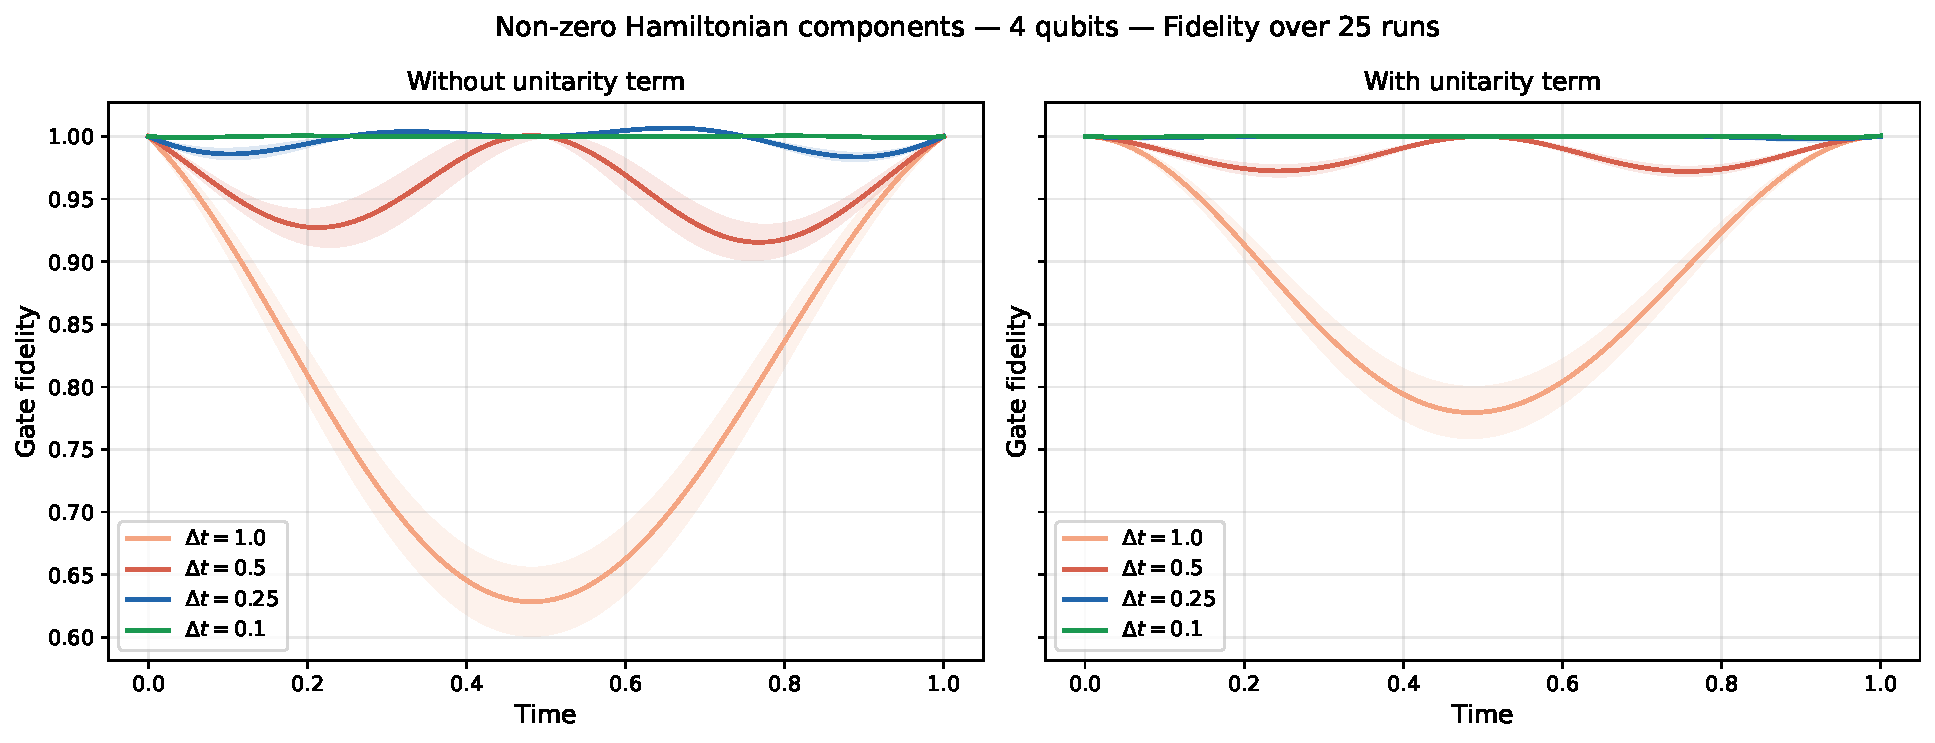
\includegraphics[width=0.88\textwidth]{images/fidelity_unitarity_N4.pdf}
\smallskip
{\small (c) Statistical analysis for the $N=4$ qubit case.}
\medskip

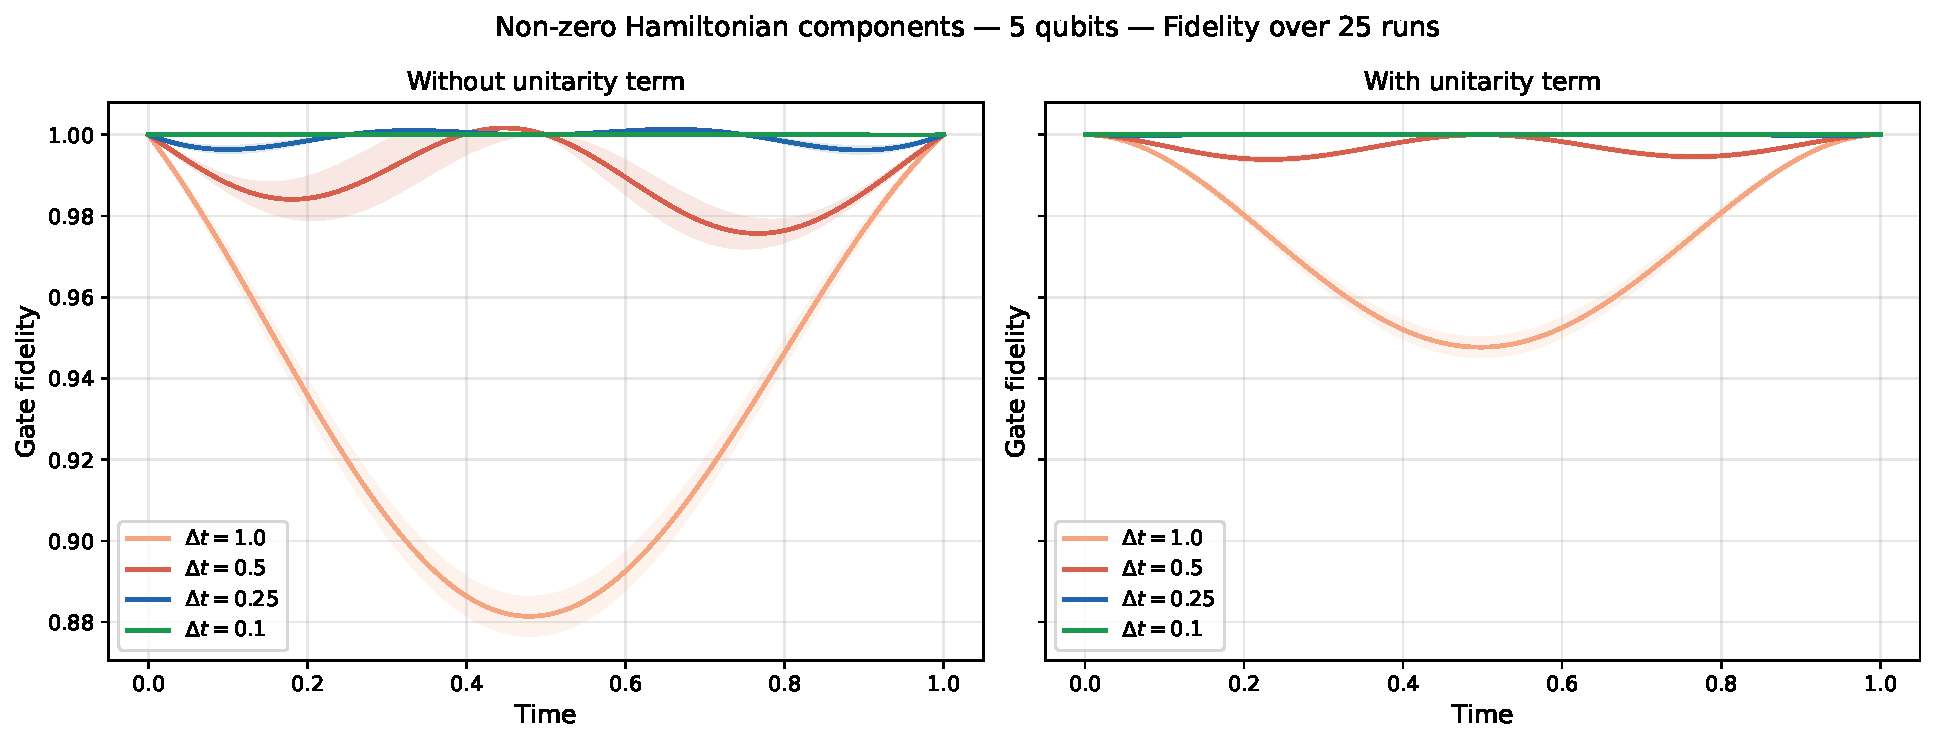
\includegraphics[width=0.88\textwidth]{images/fidelity_unitarity_N5.pdf}
\smallskip
{\small (d) Statistical analysis for the $N=5$ qubit case.}
\medskip

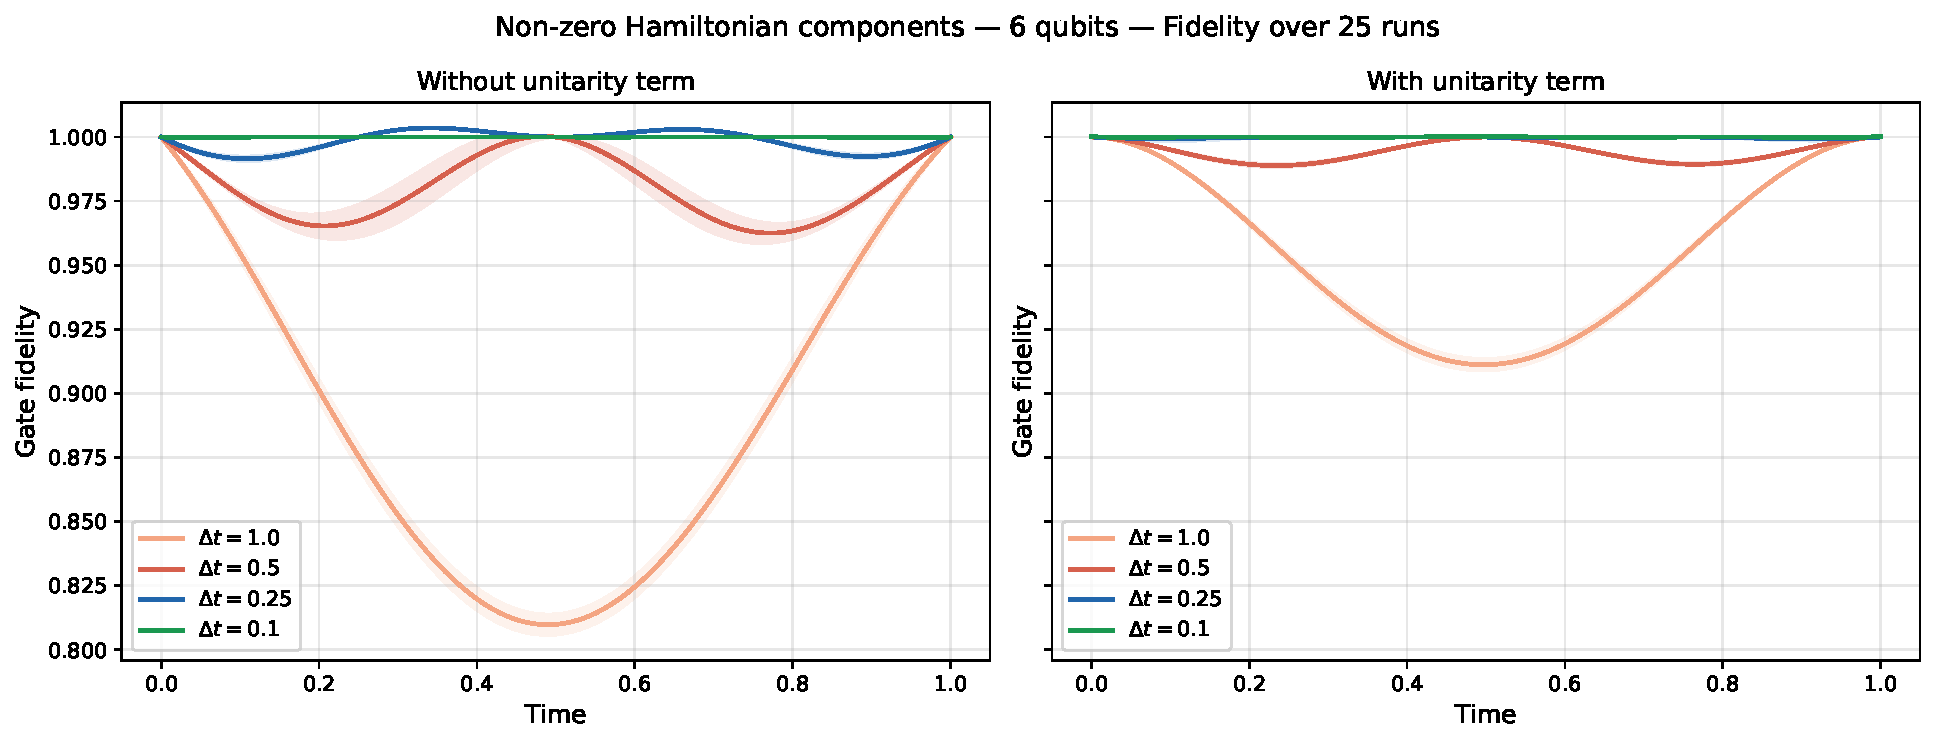
\includegraphics[width=0.88\textwidth]{images/fidelity_unitarity_N6.pdf}
\smallskip
{\small (e) Statistical analysis for the $N=6$ qubit case.}

\caption[Effect of the unitarity term in the loss function ($N=4,5,6$)]{Statistical analysis of the effect of the unitarity imposition term in the loss function over 25 independent runs for different qubit system sizes (continuation of Fig.~\ref{fig:res-unitarity-1}). In each figure, the left panel shows the results obtained without the unitarity term, while the right panel includes the additional soft constraint associated with the unitary behavior of the time-evolution operator.}
\label{fig:res-unitarity-2}
\end{figure}

\FloatBarrier

%-----------------------------------------------------------
\section{Computational time benchmark}
\label{sec:res-time-benchmark}

To assess the computational efficiency of the proposed framework, we compare the inference time of the trained PINN against the geodesic interpolation method introduced in Ref.~\cite{schilling2024}, which serves as the numerical baseline throughout this work. Given two known unitary matrices $U_0 = U(t_0)$ and $U_1 = U(t_1)$ at consecutive time points, the geodesic interpolation constructs an intermediate unitary at time $t \in [t_0, t_1]$ as
\begin{equation}
U(t) = \qty( U_1 U_0^\dagger )^\alpha U_0, \quad
\alpha = \frac{t - t_0}{t_1 - t_0},
\end{equation}
where the matrix power is computed via \texttt{fractional\_matrix\_power} from \texttt{scipy.linalg}, which relies on a Schur decomposition and scales as $\mathcal{O}(d^3)$ with the matrix dimension $d = 2^N$.

The benchmark consists of measuring the wall-clock time per query for both methods over 500 independent repetitions per system size, with query times drawn uniformly from $[0, 1]$. For systems of 7 and 8 qubits, the PINN additionally requires a numerical integration step to compute $U(t)$ from the predicted effective Hamiltonian $H_\mathrm{eff}(t)$, using either the Magnus expansion or the Trotterization. Importantly, while $r = 50$ integration steps are used during training, we find that reducing this to $r = 10$ steps at inference time does not lead to a significant loss of accuracy, since the network outputs a smooth effective Hamiltonian for which high temporal resolution is not required at evaluation time. This reduction further decreases the inference cost with respect to the training cost. In this section, all measurements for scenarios up to 5 qubits were performed on an AMD Ryzen 7 5800X, whereas those for cases of 6 qubits and above were performed on a conventional NVIDIA GeForce RTX 3060 GPU.

The results are summarized in Figs.~\ref{fig:res-timing-small} and~\ref{fig:res-timing-large}. For systems of 2 to 6 qubits, the PINN achieves speedups of $8.9\times$--$19.3\times$ over the geodesic interpolation across all system sizes, as shown in Fig.~\ref{fig:res-timing-small}. The inference time of the PINN remains nearly constant as $N$ increases, while the geodesic interpolation time grows with the matrix dimension, consistent with its $\mathcal{O}(d^3)$ scaling. For systems of 7 and 8 qubits, shown in Fig.~\ref{fig:res-timing-large}, the Trotter-based variant achieves speedups of $6.8\times$ and $17.8\times$ respectively, while the Magnus-based variant achieves $2\times$ and $7.8\times$, the latter being slower due to the additional cost of the nested commutator loop in the second-order correction. In all cases the speedup ratio exceeds unity, confirming that both PINN variants remain faster than the geodesic interpolation. This advantage is expected to grow further for larger systems where the $\mathcal{O}(d^3)$ cost of the geodesic interpolation becomes increasingly prohibitive as $d = 2^N$.

\begin{figure}[htbp]
\centering
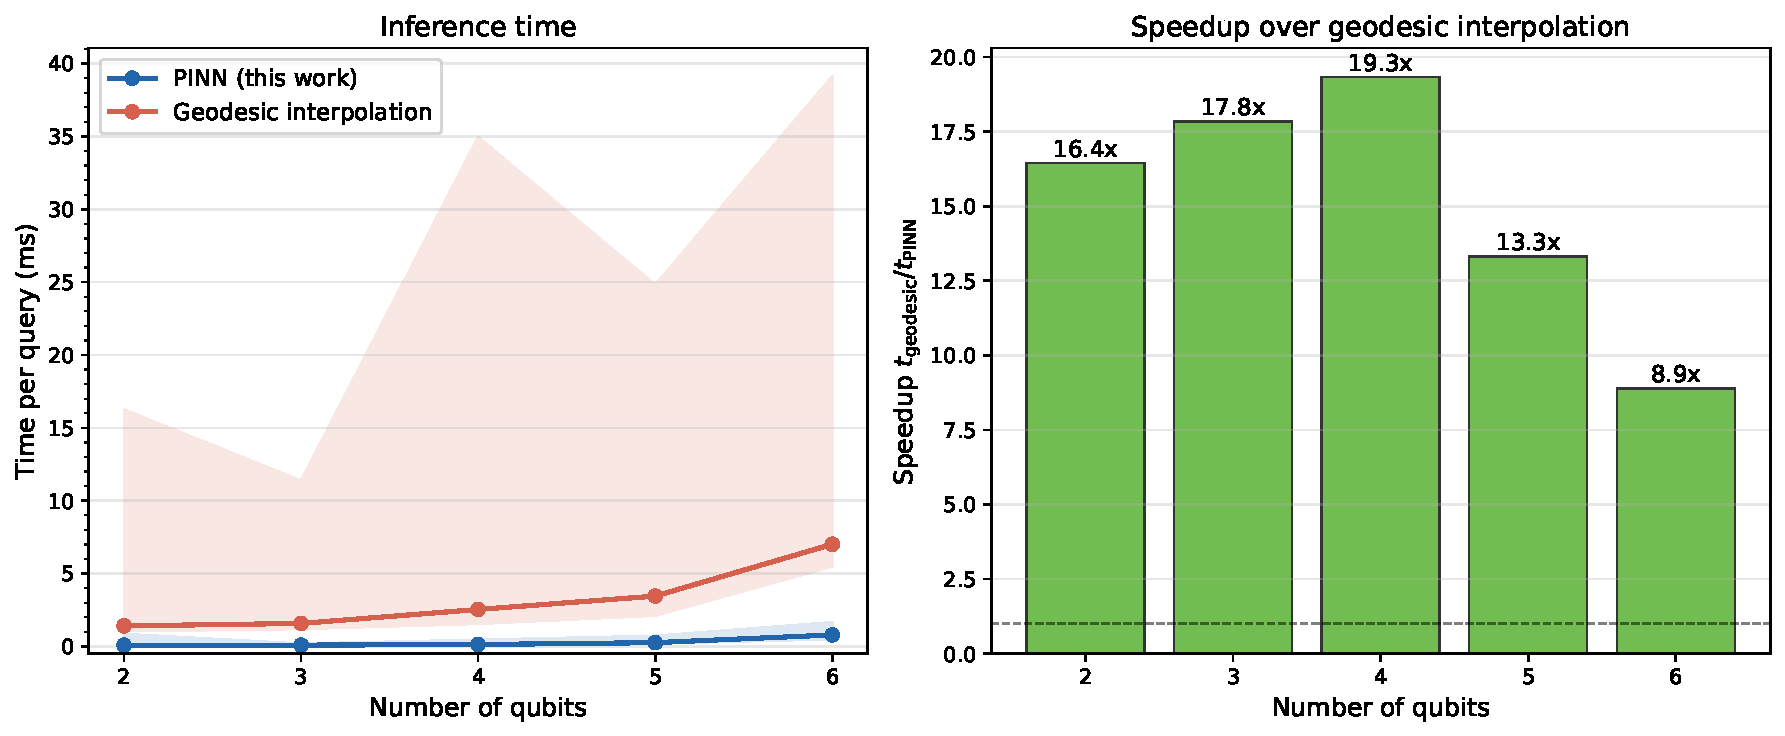
\includegraphics[width=0.99\textwidth]{images/timing_benchmark.pdf}
\caption[Timing benchmark for 2- to 6-qubit systems]{Timing benchmark for systems of 2 to 6 qubits. Left: wall-clock time per query for the PINN and the geodesic interpolation, averaged over 500 repetitions. The shaded region indicates the min/max case. Right: speedup ratio $t_\mathrm{geodesic}/t_\mathrm{PINN}$ for each system size. The dashed line indicates the break-even point at which both methods have equal cost.}
\label{fig:res-timing-small}
\end{figure}

\begin{figure}[htbp]
\centering
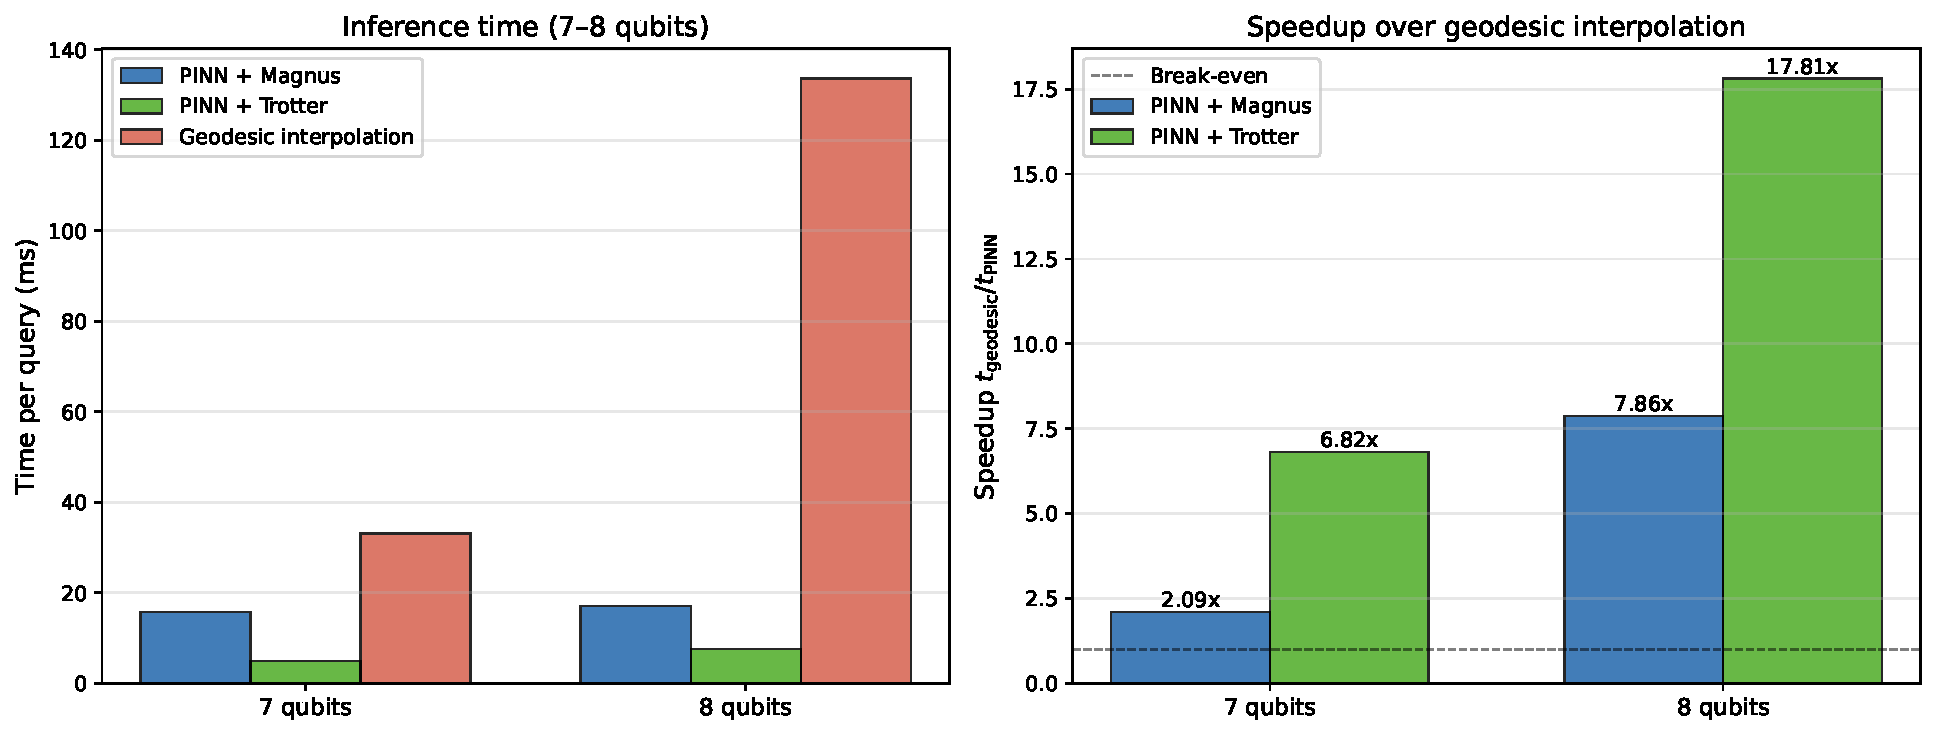
\includegraphics[width=0.99\textwidth]{images/timing_benchmark_large.pdf}
\caption[Timing benchmark for 7- and 8-qubit systems]{Timing benchmark for systems of 7 and 8 qubits. Left: wall-clock time per query for the PINN variants (Magnus and Trotter) and the geodesic interpolation, averaged over 500 repetitions with $r = 10$ integration steps at inference time. Right: speedup ratio $t_\mathrm{geodesic}/t_\mathrm{PINN}$ for each variant. The dashed line indicates the break-even point.}
\label{fig:res-timing-large}
\end{figure}

\FloatBarrier

%-----------------------------------------------------------
\section{Summary}
\label{sec:res-summary}

The results presented in this chapter show that PINNs can accurately interpolate the quantum dynamics encoded in the training data. Across all system sizes, the framework achieved mean gate fidelities close to $0.99$ with low variability across independent Hamiltonian realizations, and models trained with coarse temporal sampling ($\Delta t = 1.0$) reproduced the dynamics almost as well as those trained with fine grids, confirming a strong interpolation capability that reduces the associated measurement cost. The trace-distance analysis confirmed accurate state reconstruction across the considered range of system sizes, and the timing benchmark showed inference times substantially below those of the geodesic-interpolation baseline~\cite{schilling2024}, an advantage expected to grow with system size.

The framework also has well-defined limitations: a dedicated model must be trained for each Hamiltonian and system size, and the learned effective Hamiltonian for the 7- and 8-qubit cases captures the dynamics without coinciding with the true generator. These limitations, together with the broader implications of this work for large-scale quantum information and its connection to the marginal-reconstruction framework of Chapter~\ref{ch:results-qmp}, are discussed in the general conclusions of Chapter~\ref{sec:conclusions}.
